\subsection{Reviving the VIPUR approach to expand rare disease diagnostics}
	\subsubsection{Preparatory steps for using the VIPUR approach}
		After the publication of VIPUR the tools, data and applications became available at the open science framework (OSF) \cite{baugh_vipur:_2015} which were downloaded and reviewed. All applications from the Rosetta software suite (Section \ref{subsec:MM_Rosetta}) were pre-compiled without support for MPI (Section \ref{subsec:MM_MPI}) and with that not the ability to benefit from multiple CPUs. The Rosetta software suite was rebuilt with MPI support in a slurm job where the compilation could benefit from multiple CPU cores.
		%VIPUR: Variant Interpretation and Prediction Using Rosetta, Baugh
	\label{subsubsec:RES_Prepare}
	
	\subsubsection{Resolving VIPUR system incompatibilities}
	Within the VIPUR pipeline residues were mutated to determine the effects of a structural mutation, by default missense mutations were inserted with PyMOL (Section \ref{subsec:MM_PyMOL}), an alternative method integrated within the pipeline for situations wherein PyMOL was not accessible Pyrosetta (Section \ref{subsec:MM_PyRosetta}) could be used. Neither of these programs could be built or compiled because the lack of Open graphics library (OpenGL) for PyMOL and having the incorrect C++ and C libraries for PyRosetta. To bypass both programs and still be able to introduce mutations into PDB files Modeller (Secton \ref{subsec:MM_Modeller}) was introduced and built.
	
	\begin{figure}[!ht]
		\centering
		\begin{subfigure}{0.45\textwidth}
			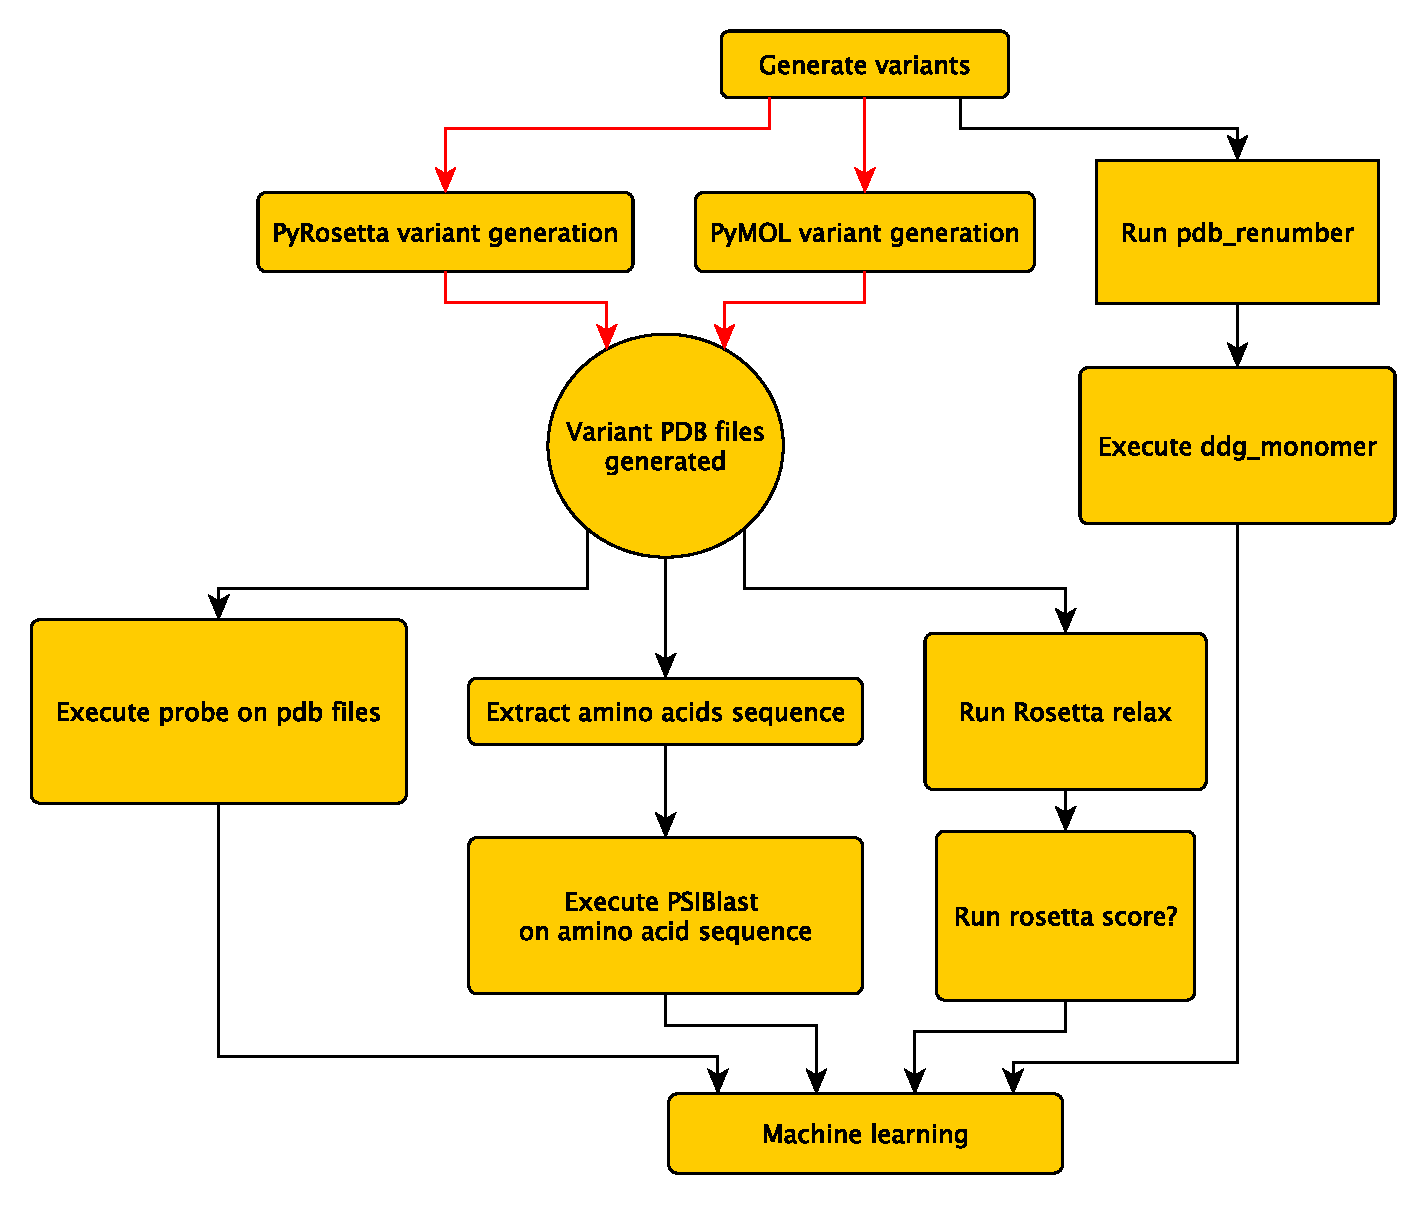
\includegraphics[width=\textwidth,height=0.3\textheight]{Flowcharts/VIPUR_approach.pdf}
			\caption{Original VIPUR approach}
			\label{fig:RES_VIPUR_approach}
		\end{subfigure}
		\begin{subfigure}{0.45\textwidth}
			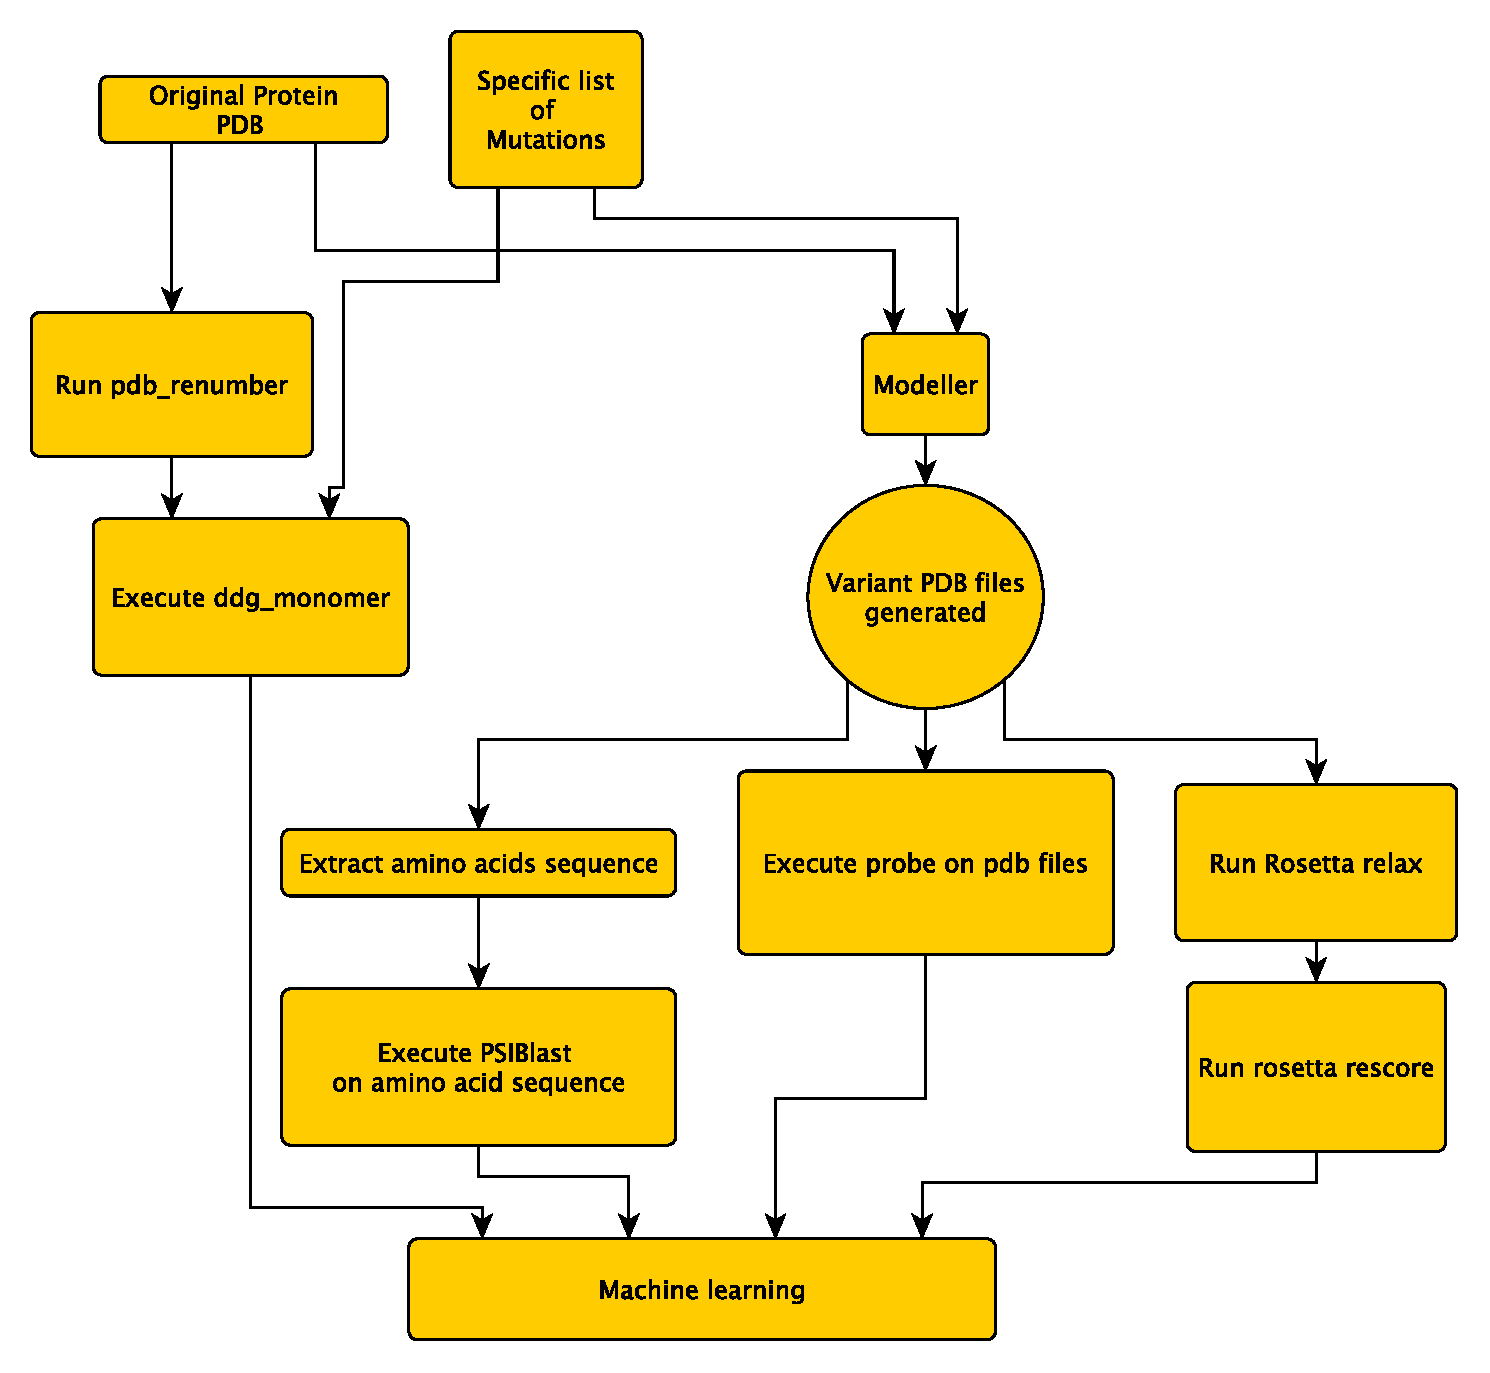
\includegraphics[width=\textwidth,height=0.3\textheight]{Flowcharts/Altered_VIPUR_approach.pdf}
			\caption{Altered VIPUR approach}
			\label{fig:RES_Altered_VIPUR_approach}
		\end{subfigure}
		\caption[Flowcharts VIPUR pipeline and altered VIPUR pipeline]{Both flowcharts illustrate the VIPUR pipeline wherein each block is a procedure the central circle is the purpose of the mutated applications and each arrow represents the path to it. Figure \ref{fig:RES_VIPUR_approach} has red arrows that indicate that both methods were incapable to produce the mutated PDB files. Within figure \ref{fig:RES_Altered_VIPUR_approach} the alternative method is proposed wherein PyMOL and PyRosetta (Sections \ref{subsec:MM_PyMOL}, \ref{subsec:MM_PyRosetta}) is substituted by Modeller (Section \ref{subsec:MM_Modeller}) to acquire the mutated protein structures.(To zoom in on the details within the figure it is recommend to look at the PDF version.)}

		\label{fig:Flowcharts_of_old_and_altered_VIPUR}
	\end{figure}
	\label{subsubsec:RES_Incompatibility}
	\newpage
	
	\subsubsection{Expanding the VIPUR training set with data from TNFRSF1A by homology modeling and protein threading}
	Since the VTS did not have any features of TNFRSF1A (Section \ref{subsec:CD_TNFRSF1A}) the amino acid sequence was collected from Uniprot (Section \ref{subsec:MM_Uniprot}) and the protein from RCSB (Section \ref{subsec:MM_RCSB}). The structures available of TNFRSF1A were incomplete, fragments for the TNF $\alpha$ and $\beta$ binding site \cite{banner_crystal_1993} were available and its death domain that interacts with TRADD \cite{sukits_solution_2001} which plays a role in apoptosis (Section \ref{subsec:CD_TNFRSF1A}). To acquire a monomeric structure of TNFRSF1A two ab initio modeling web services I-TASSER and Robetta (Sections \ref{subsec:MM_I_TASSER}, \ref{subsec:MM_Robetta}) had been employed. Both were given the task to model the whole protein with and without a template to determine how well they could model a known structure and what it would form. Determination of the best model was based on the smallest root mean square deviation distance (RMSD )in {\AA} , between a produced model compared to the X-ray crystallographic model of the TNFRSF1A binding site.
	
%	Solution structure of the tumor necrosis factor receptor-1 death domain, Sukits
	\begin{figure}[!ht]
		\centering
		\begin{subfigure}{0.49\textwidth}
			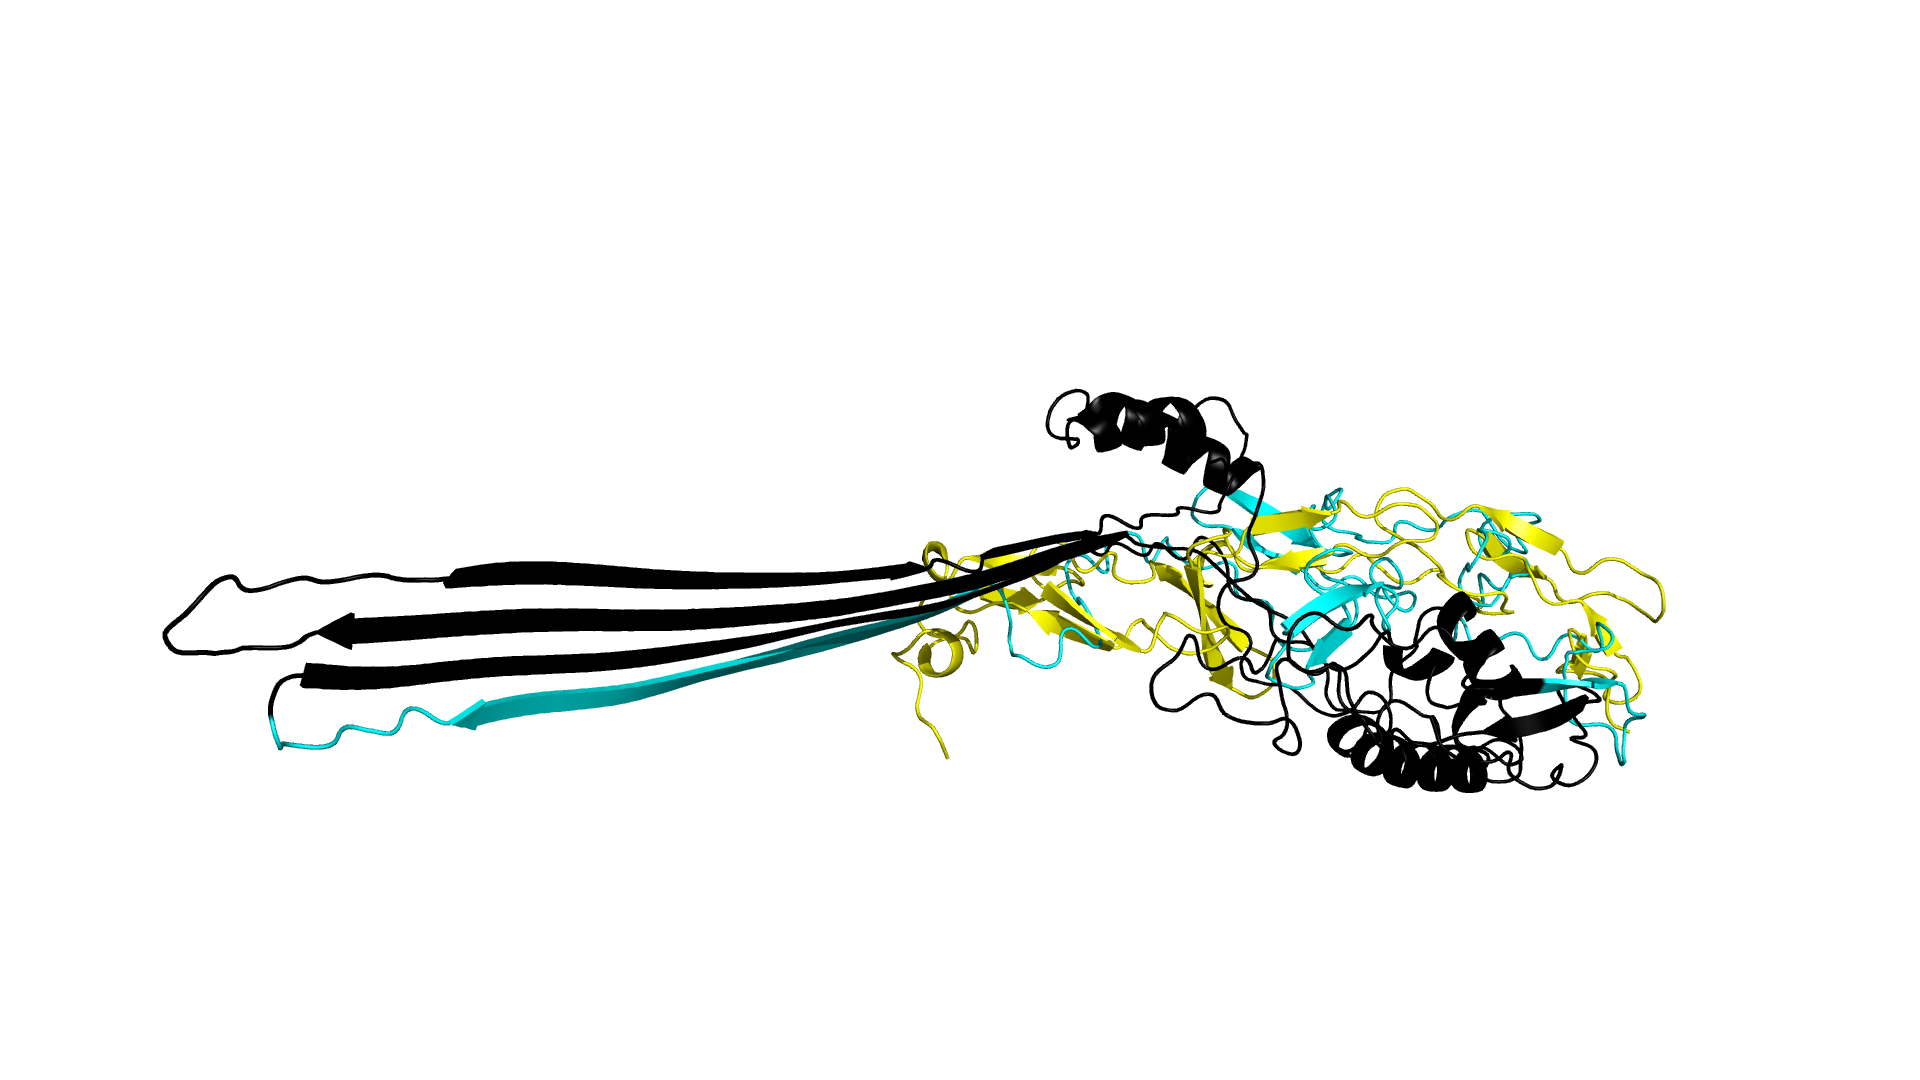
\includegraphics[width=\textwidth]{I_TASSER_Robetta_Images/1_EXT_ALIGN_I_TAS_WITHOUT_TEMPLATE.png}
			\caption{RMSD = {\AA} 28.786}
			\label{fig:RES_I_TASSER_Without}
		\end{subfigure}
		\begin{subfigure}{0.49\textwidth}
			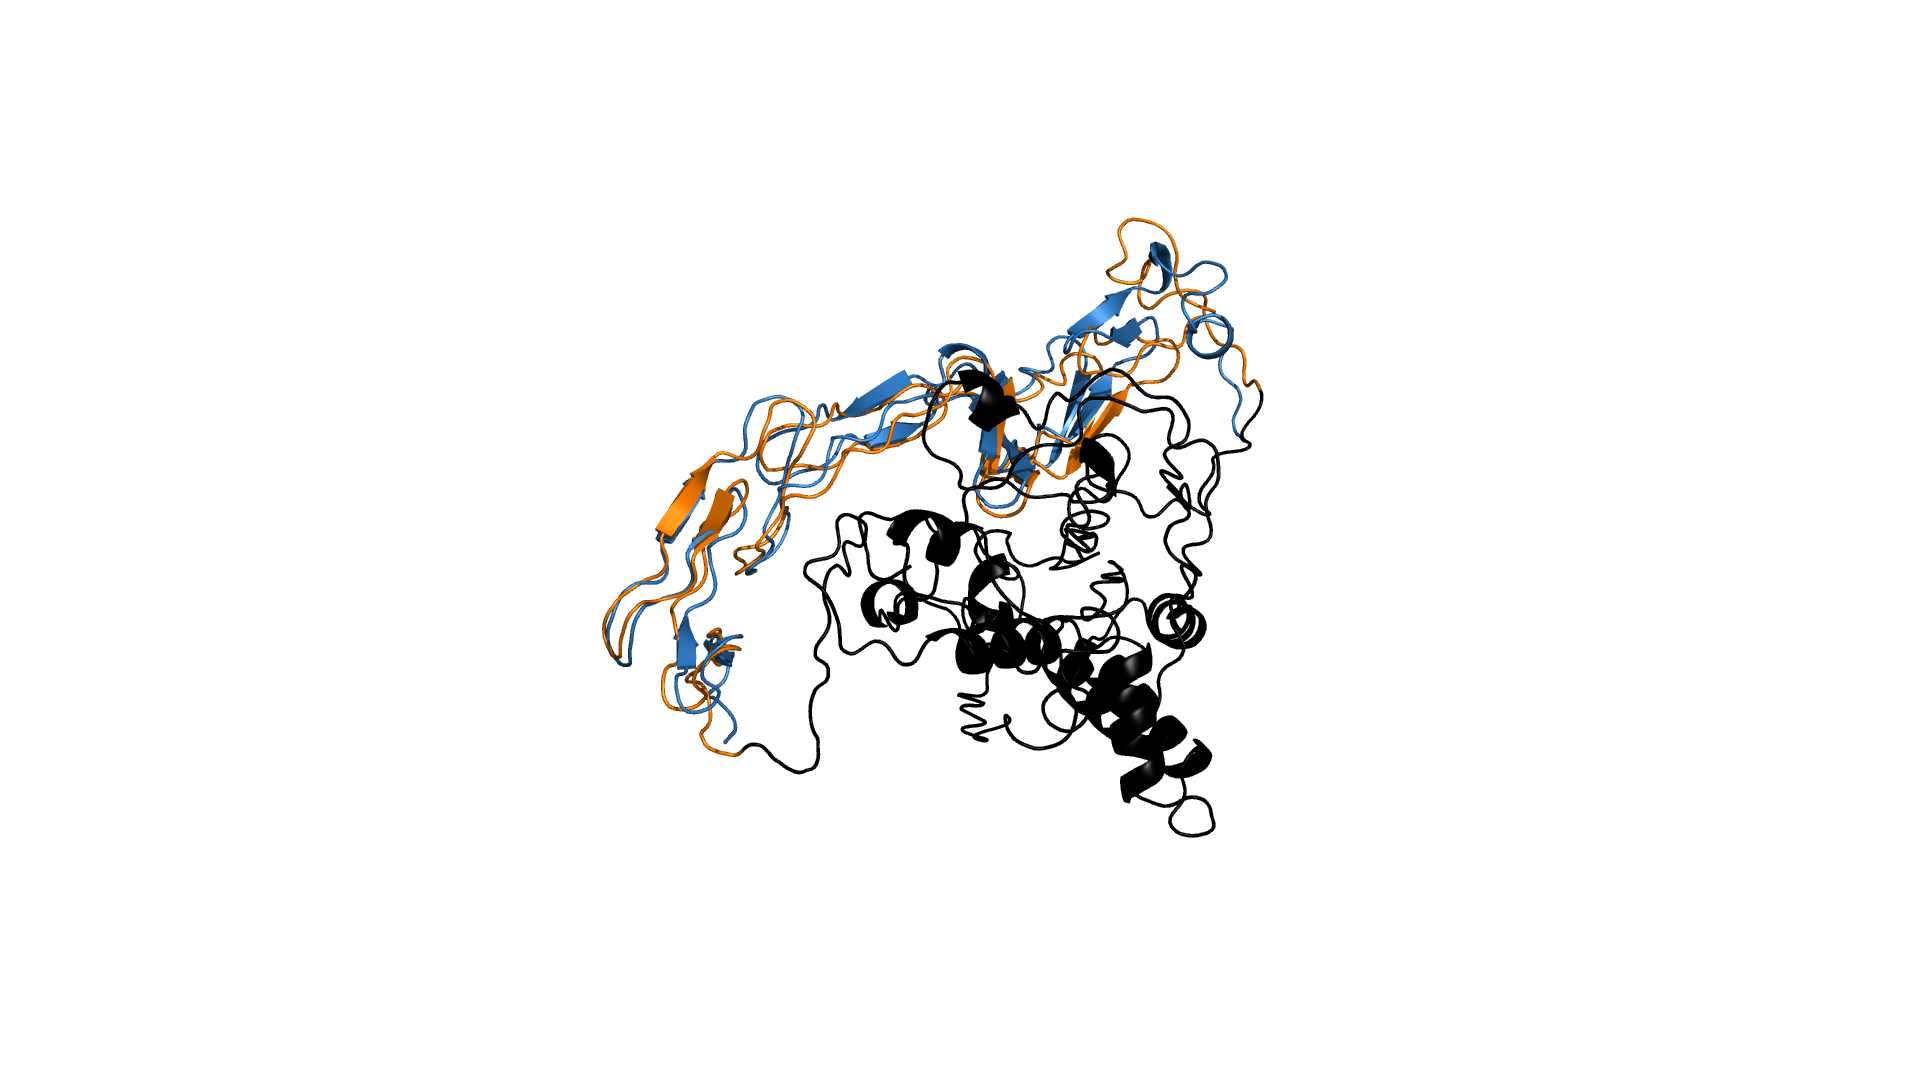
\includegraphics[width=\textwidth]{I_TASSER_Robetta_Images/1_EXT_ALIGN_I_TAS_WITH_TEMPLATE.png}
			\caption{RMSD = {\AA} 3.830}
			\label{fig:RES_I_TASSER_With}
		\end{subfigure}
		\par\bigskip
		\begin{subfigure}{0.49\textwidth}
			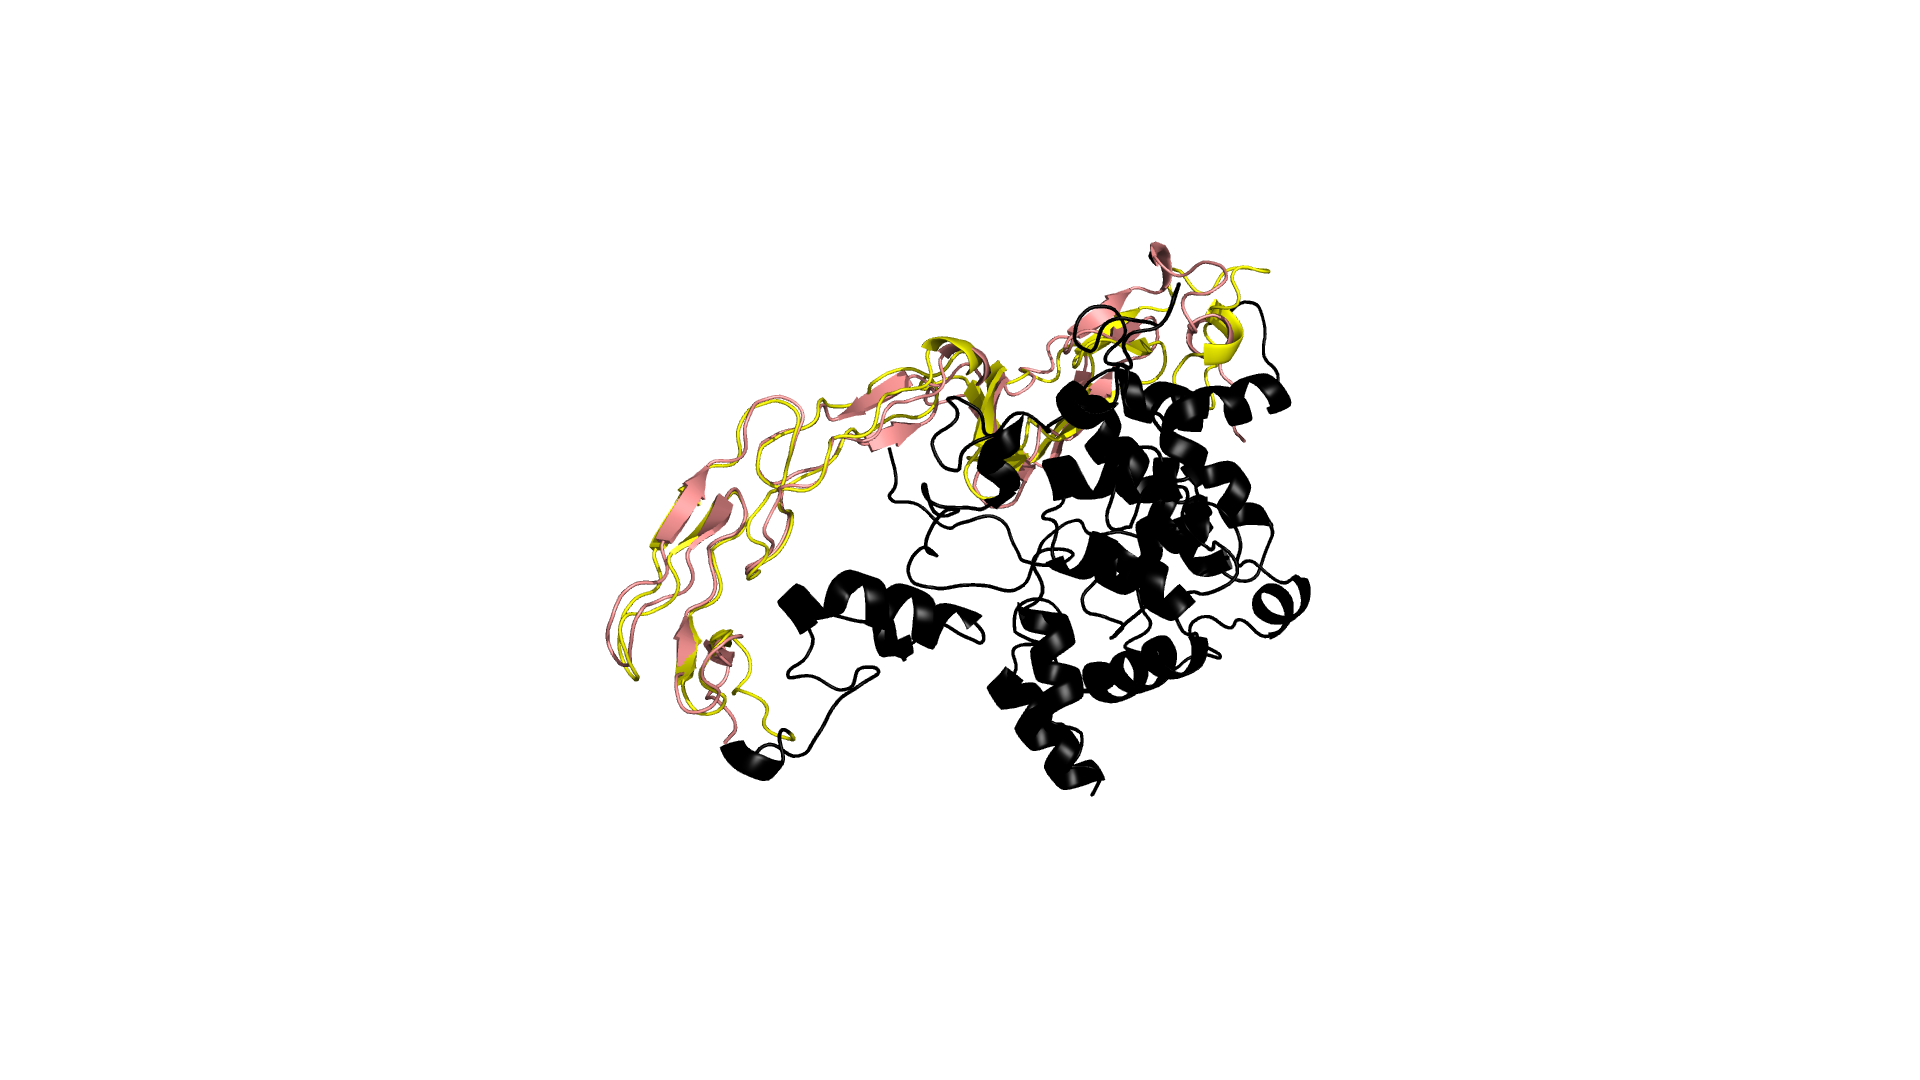
\includegraphics[width=\textwidth]{I_TASSER_Robetta_Images/1_EXT_ALIGN_ROB_WITHOUT_TEMPLATE.png}
			\caption{RMSD =  {\AA} 3.067}
			\label{fig:RES_Robetta_Without}
		\end{subfigure}
		\begin{subfigure}{0.49\textwidth}
			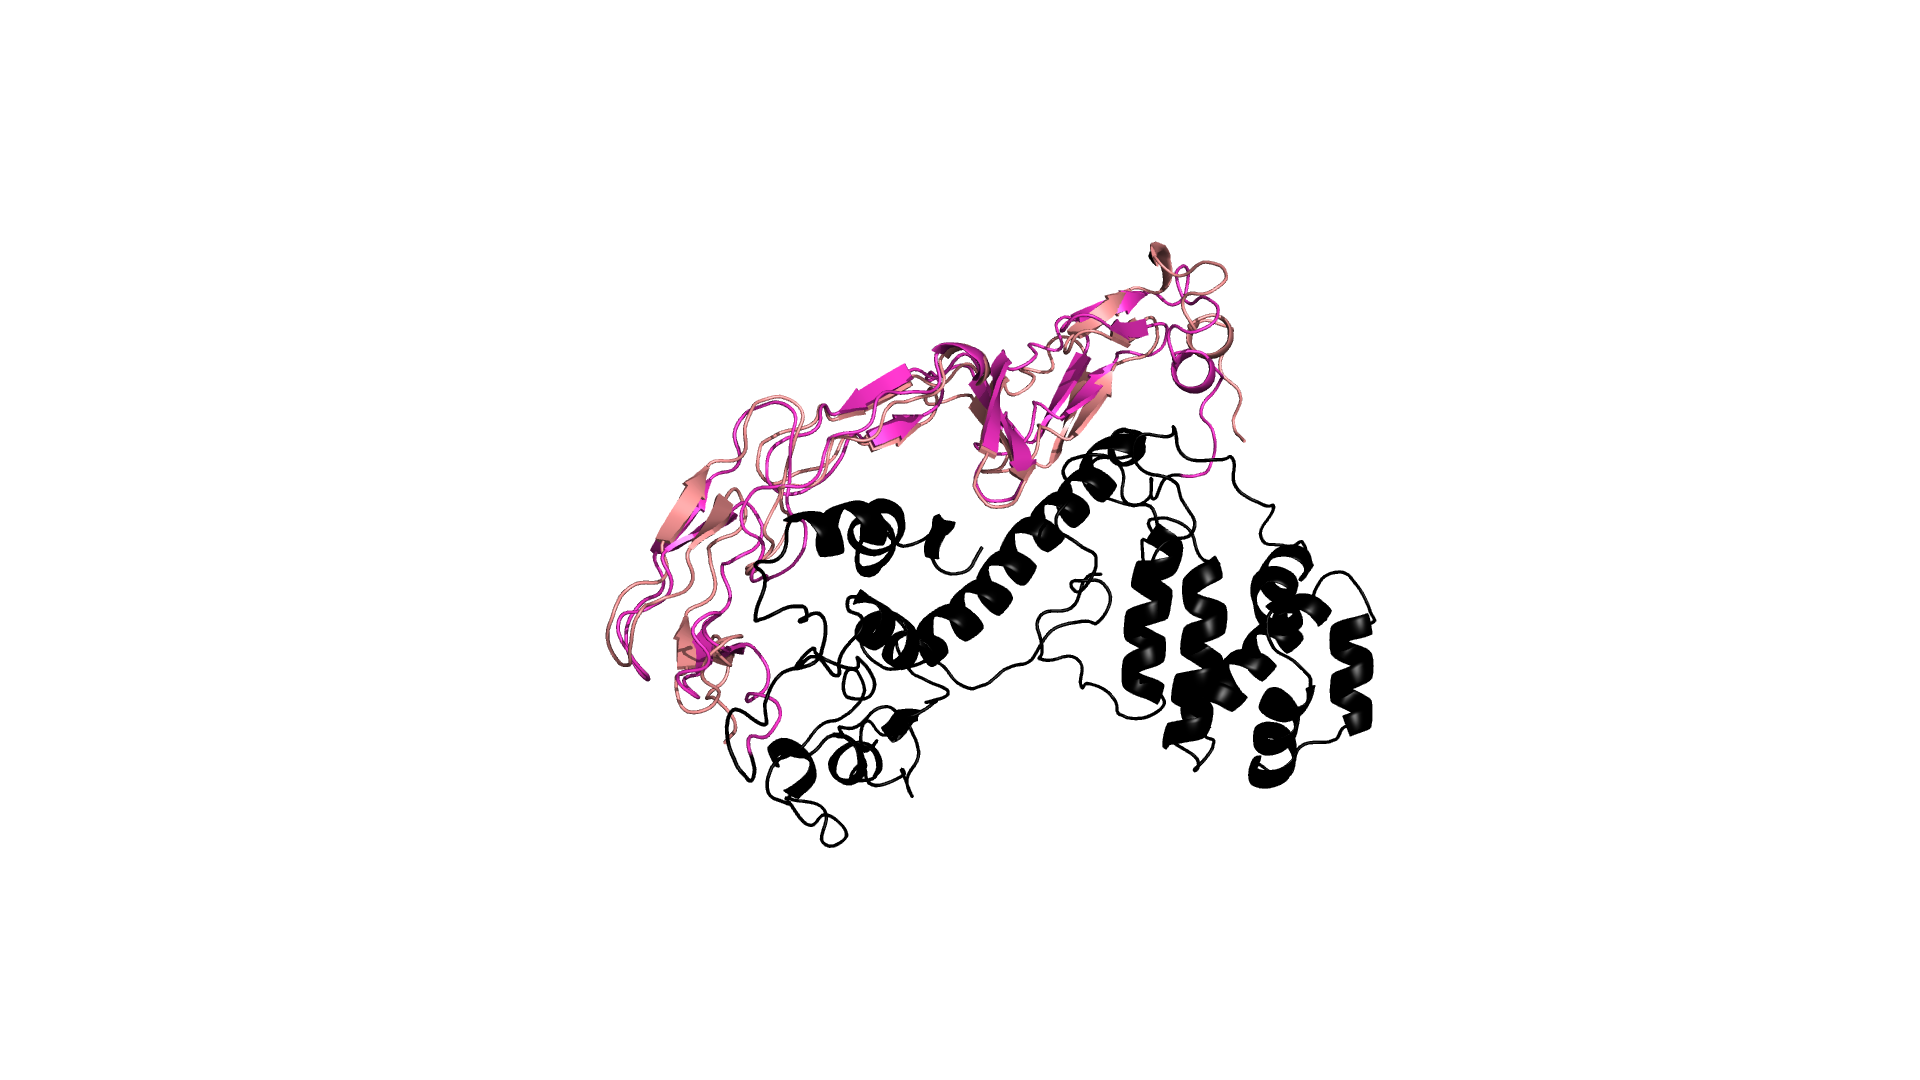
\includegraphics[width=\textwidth]{I_TASSER_Robetta_Images/1_EXT_ALIGN_ROB_WITH_TEMPLATE.png}
			\caption{RMSD =  {\AA} 2.877}
			\label{fig:RES_Robetta_With}
		\end{subfigure}
		\caption[I-TASSER and Robetta models with and without templates]{3D structures of TNFRSF1A ( \ref{fig:RES_I_TASSER_Without}, \ref{fig:RES_I_TASSER_With}: I-TASSER, \ref{fig:RES_Robetta_Without}, \ref{fig:RES_Robetta_With}: Robetta) without (left: \ref{fig:RES_I_TASSER_Without}, \ref{fig:RES_Robetta_Without}) and with templates (right: \ref{fig:RES_I_TASSER_With}, \ref{fig:RES_Robetta_With}). The sky blue colored structure in each figure is an X-ray crystallographic model (1EXT) of the binding site of TNFRSF1A and the orange structure is the representation of that identical fragment in the model made by the web services.(To zoom in on the details within the figure it is recommend to look at the PDF version.)}
		\label{fig:I_Tasser_Robetta_models}
	\end{figure}
	\label{subsubsec:RES_Expanding_Models}
	
	\subsubsection{Practical VIPUR usage}
	With the hindrance of software incompatibility on the cluster, difference in produced models between the web services, discovery of consequences by removing elements from structures, and the time it would take to reverse engineer VIPUR a new decision was formed. VIPUR would be set aside for now and if time was left there would be further looked into to make it applicable for protein structure evaluation.

\newpage
\subsection{Analyses of proteins variants TNFRSF1A}
	\subsubsection{Requirements for determining structural and binding effects of protein variants}
	Protein variants can be assessed from multiple perspectives and together they can form a holistic view on how a protein works and how mutations affect its workings. However adding perspectives to the protein assessment makes it complex and requires expertise to determine its validity and contribution, therefore the analysis has been limited to basic structural information and also make the assessment inline with the VIPUR methods.
	
	Various proteins consist of multiple chains that can be identical or different depending on their function \cite{liu_lipin_2010} and should be taken into account when assessing protein variants since one residue might alter the binding between chains and might alter the proteins formation. 
%	Lipin proteins form homo- and hetero-oligomers, Liu et al.
	Different molecules and atoms that do not make up a protein but play a role in a pathway and function (ligands and co-receptors) are able to affect a proteins shape and can behave differently when a residue is mutated. 
	
	A different aspect that can change with mutations is the alteration in motions between structures which can allow or disallow certain movements to occur and with inhibit processes.
	
	\subsubsection{Introduction of the simple protein variant analysis approach}
	A different method for determining function loss in a protein variant is through assessment of difference in energy levels between a wild type and a variant in the complex where it resides. Analyzing mutations from this perspective gives the ability to view a protein in whole and determine how residues cause perturbations in a protein. To make a variant of the wild type, a structure was required wherein a missense mutation could be introduced with Modeller (Section \ref{subsec:MM_Modeller}). The backbone structure of the variant was modified with the backrub application (Section \ref{subsubsec:MM_Backrub}) to make it better interact with other amino acid backbones in the structure resulting in 1000 models. The lowest Rosetta scoring (Section \ref{subsec:MM_Rosetta}) one would be selected to further improve the side chains with the Relax application	(Section \ref{subsubsec:MM_Relax}) which makes the side chains of the protein move into lower energy formations. From these 64 models were made where its energies levels were compared to the native structure to determine the effects a mutation would have on the protein, the lowest scoring ones were used as figures. This method shows similarities to that of VIPUR and was only tested on TNFRSF1A (Section \ref{subsec:CD_TNFRSF1A}) and its ligands TNF $\alpha$ and $\beta$. This method keeps: duplicate chains and protein ligands within the structure, water is excluded since it can cause issues with Rosetta tools (Section \ref{subsec:MM_Rosetta}). This procedure with these steps is defined as the Simple protein variant analysis approach (SPVAA).
	
	\begin{figure}[!ht]
		\centering
		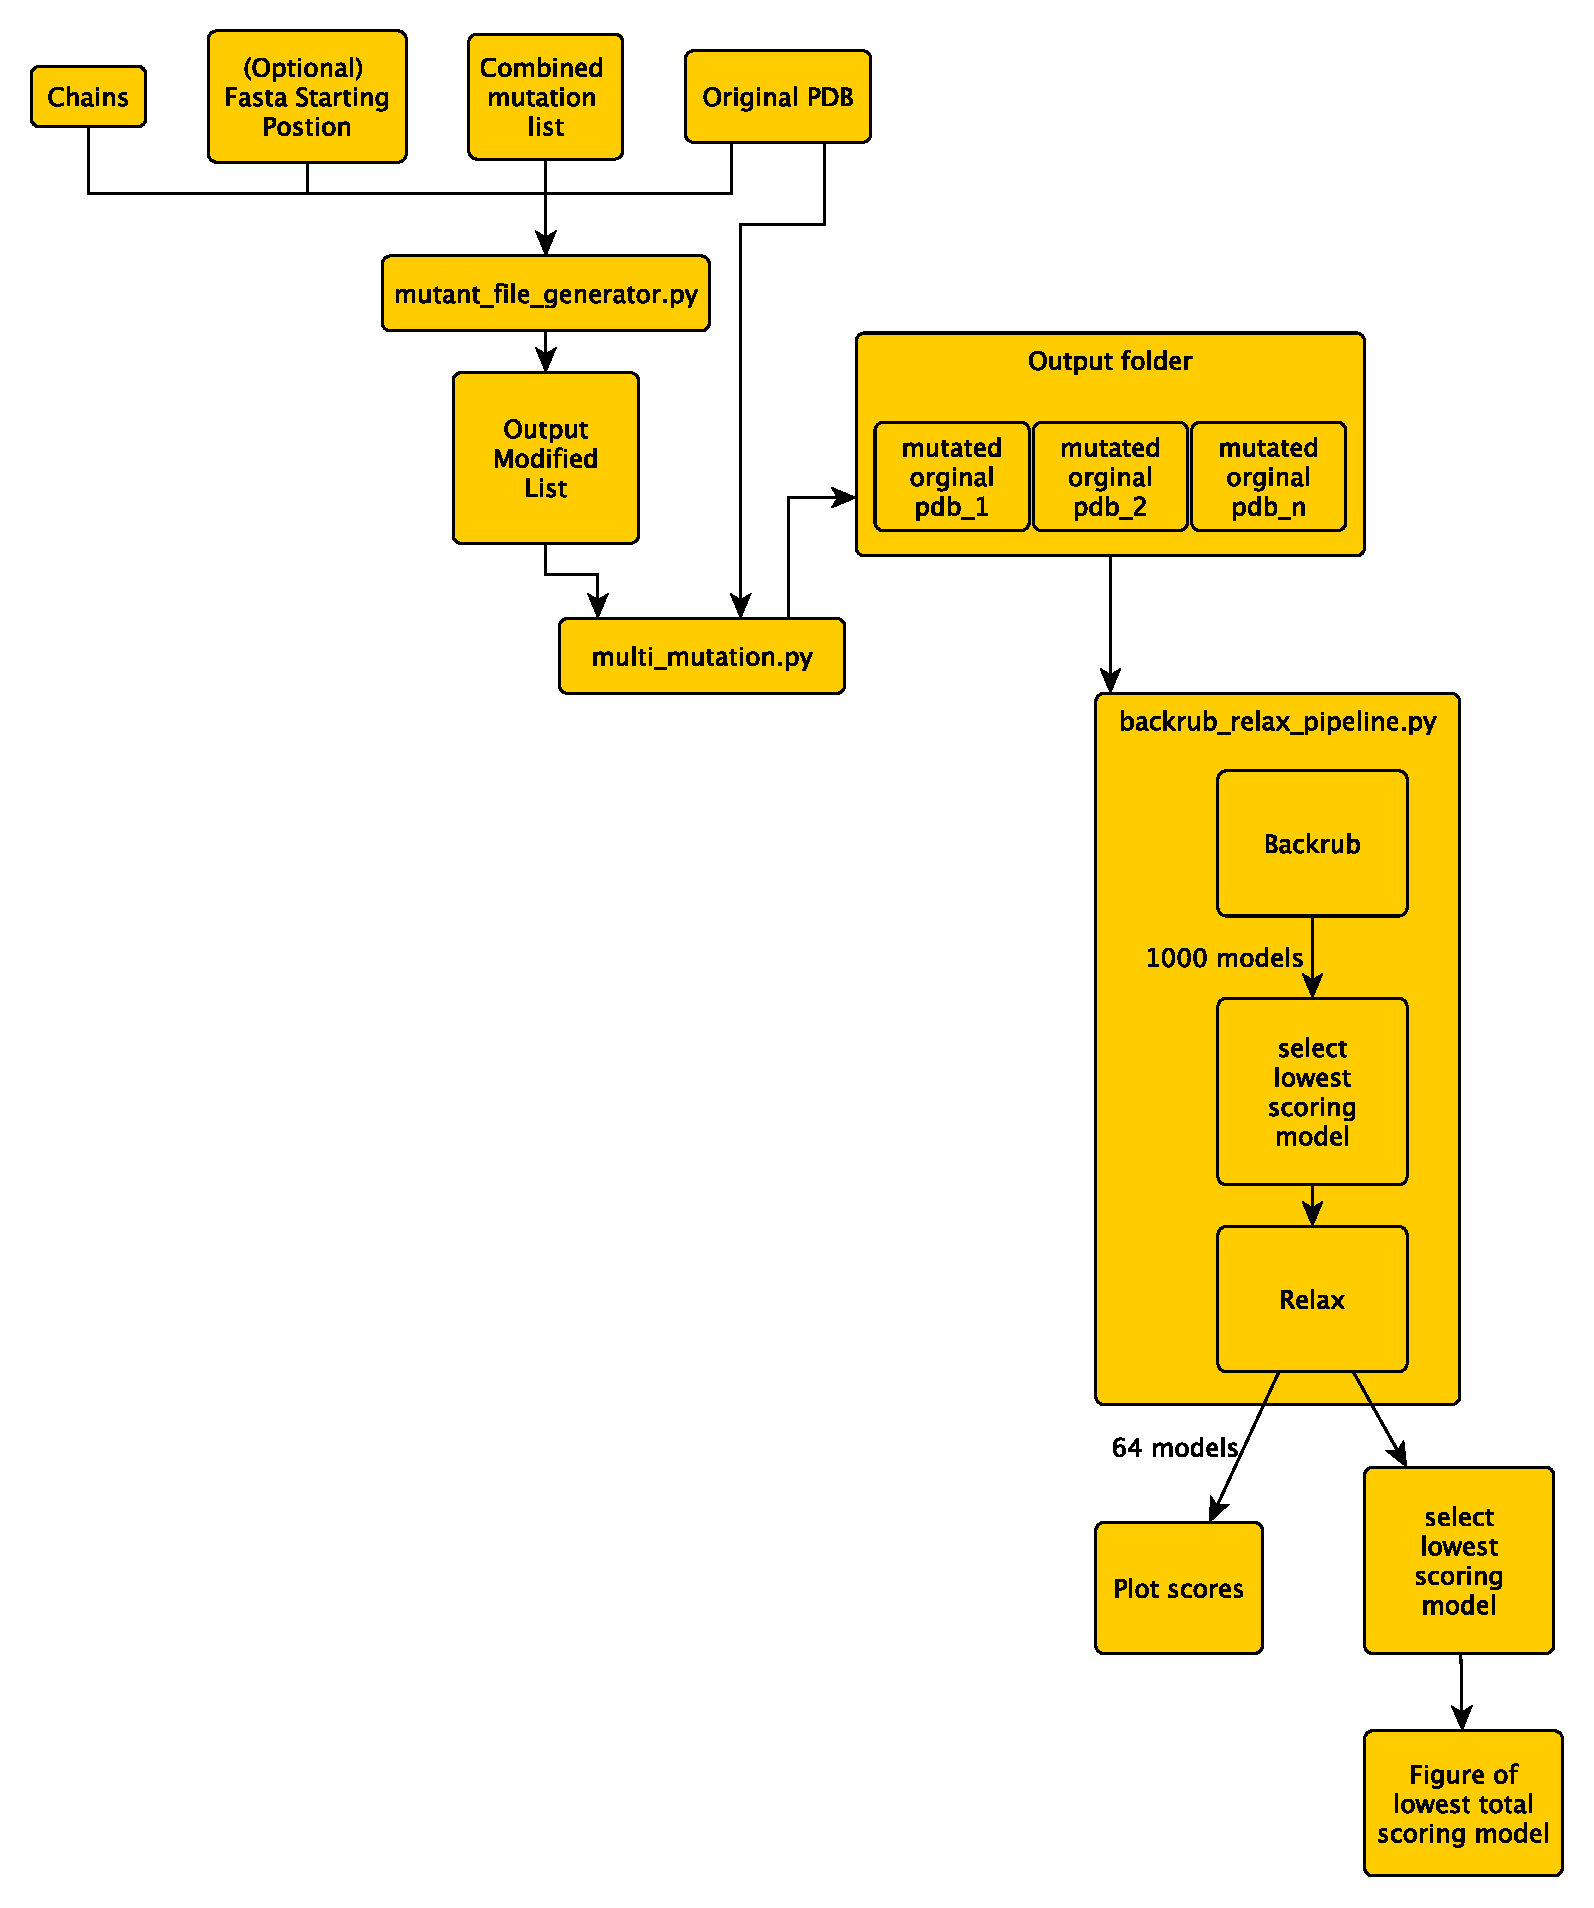
\includegraphics[width=0.5\textwidth]{Flowcharts/SPVAA_pipeline.pdf}
		\caption[Flowchart SPVAA pipeline]{Flowchart of SPVAA wherein a list of known mutations generate the appropriate information for modeller to mutate residues in the original PDB of the protein and feed it into the backrub relax pipeline where the model is altered to go into a lower energy state.(To zoom in on the details within the figure it is recommend to look at the PDF version.)}
	\end{figure}
	\newpage
	
	\subsubsection{Carrying out SPVAA on TNFRSF1A}
	Before introducing mutations into a protein structure it is helpful to know if a mutation has been observed to avoid allocating resources to something that does not occur. Therefore three tables with observed TNFRSF1A mutations (Sections \ref{subsec:MM_GAVIN_data_table}, \ref{subsec:MM_GnomAD}, \ref{subsec:MM_Infevers}) have been combined with an R script (Section \ref{subsec:MM_R}) into a single table consisting of two columns. The first column (split into three columns \ref{table:Res_Filtered_Mutations}) contains strings that describes the: original residue, position and where it mutates to, the second column describes whether a formed mutation is harmful, with most mutations the effects have not been identified yet. 
	\begin{table}[ht]
		\begin{tabular}{ l | l | l | l}
			Original residue & Position in the protein sequence & New residue & Classification\\ \hline
			Cys & 44 & Tyr & PATHOGENIC\\
			Thr & 44 & Pro & PATHOGENIC\\
			Thr & 44 & Ser & PATHOGENIC\\
		\end{tabular}
		\caption[Sample from the combined observed TNFRSF1A mutations table]{The format wherein mutations were filtered from the GAVIN, GenomAD and Infevers tables (Sections \ref{subsec:MM_GAVIN_data_table},  \ref{subsec:MM_GnomAD}, \ref{subsec:MM_Infevers}),  describe whether a structural mutation is harmful or not. For many mutations it is unknown and other classifications are available, to view the whole table visit the supplementary.}
		\label{table:Res_Filtered_Mutations}
	\end{table}
	
	For assessing variants in TNFRSF1A a structural fragment was used that contained TNF $\beta$ (1TNR) \cite{banner_crystal_1993} and was made homotrimeric with PyMOL (Section \ref{subsec:MM_PyMOL}) which results in six chains that emulate a bound TNFRSF1A with TNF $\beta$. The first column of the mutation table did not contain sufficient information to apply mutations correctly and within the PDB different numbering is used than in the amino acid sequence. To bundle the information and make it usable for introducing mutations a Python script (Section \ref{subsec:MM_Python}) has been written that combines the mutation table, PDB chains and the correct position within the sequence into a type of table which has sufficient information to mutate structures.  
	%	Crystal structure of the soluble human 55 kd TNF receptor-human TNFβ complex: Implications for TNF receptor activation, Banner et al. 
	\begin{table}[ht]
		\begin{tabular}{ l | l | l | l | l}
			Iteration number & Filename & Chain & Residue index in chain & New residue\\ \hline
			34 & 1tnr3\_TNFA & R & 0 & TYR\\
			34 & 1tnr3\_TNFA & T & 0 & TYR\\
			34 & 1tnr3\_TNFA & S & 0 & TYR\\
			35 & 1tnr3\_TNFA & R & 0 & PRO\\
			35 & 1tnr3\_TNFA & T & 0 & PRO\\
			35 & 1tnr3\_TNFA & S & 0 & PRO\\
			36 & 1tnr3\_TNFA & R & 0 & SER\\
			36 & 1tnr3\_TNFA & T & 0 & SER\\
			36 & 1tnr3\_TNFA & S & 0 & SER\\
		\end{tabular}
		\caption[Sample of the TNFRSF1A PDB residue mutation table]{The format that describes the mutations that should be made by Modeller (Section \ref{subsec:MM_Modeller}), with specifications of the: model, file. chain, residue index and the new residue. The whole table for TNFA and TNFB are visible within the supplementary.}
			\label{table:Res_Modeller_Mutation_Format}
	\end{table}
	
	To introduce mutations within PDB structures a Python script (Section \ref{subsec:MM_Python}) was written which used the generated mutation table (Table: \ref{table:Res_Modeller_Mutation_Format}) and a matching PDB structure, from the table; it acquires an iteration number which specifies if a mutation has to be stored in a single file or across multiple files; the filename serves as key which determine the PDB that should be used; letters specify chains, numbers are indices within the chains and the last column states the three letter residue where it should mutate to. When a structure is read in through the Python bindings of Modeller (Section \ref{subsec:MM_Modeller}) all non standard atoms and molecules are removed because Rosetta (Section \ref{subsec:MM_Rosetta}) is not able to deal with those atoms. Just before mutagenesis takes place missing atoms are added to the structure that were difficult to determine with experimental methods(Section \ref{subsec:GD_Addition_of_structural_data}). After the insertion of all mutations a last attempt was made by modeller to add dislufide bridges, based on the distance between cysteine residues, into the structure.
	
	With the many protein variants generated and limited resources to use SPVAA mutations had to be chosen. All mutations were picked from the Infevers table because that were variants of a single isoform and had a protein structure (1TNR \cite{banner_crystal_1993}) available that interacted with TNF $\beta$. 
	%Crystal structure of the soluble human 55 kd TNF receptor-human TNFβ complex: Implications for TNF receptor activation, Banner
	Mutations cysteine 62 to glycine and phenylalaine acid 141 to isoleucine were validated as pathogenic mutations within Infevers table and were used to determine the effectiveness of SPVAA. Within the infevers table no benign validated missense mutations were available, but to still have the opportunity to asses a likely benign mutation, the mutation glutamic acid 138 to alanine has been added to SPVAA.	
	
	\newpage
	\begin{figure}[!ht]
		\centering
		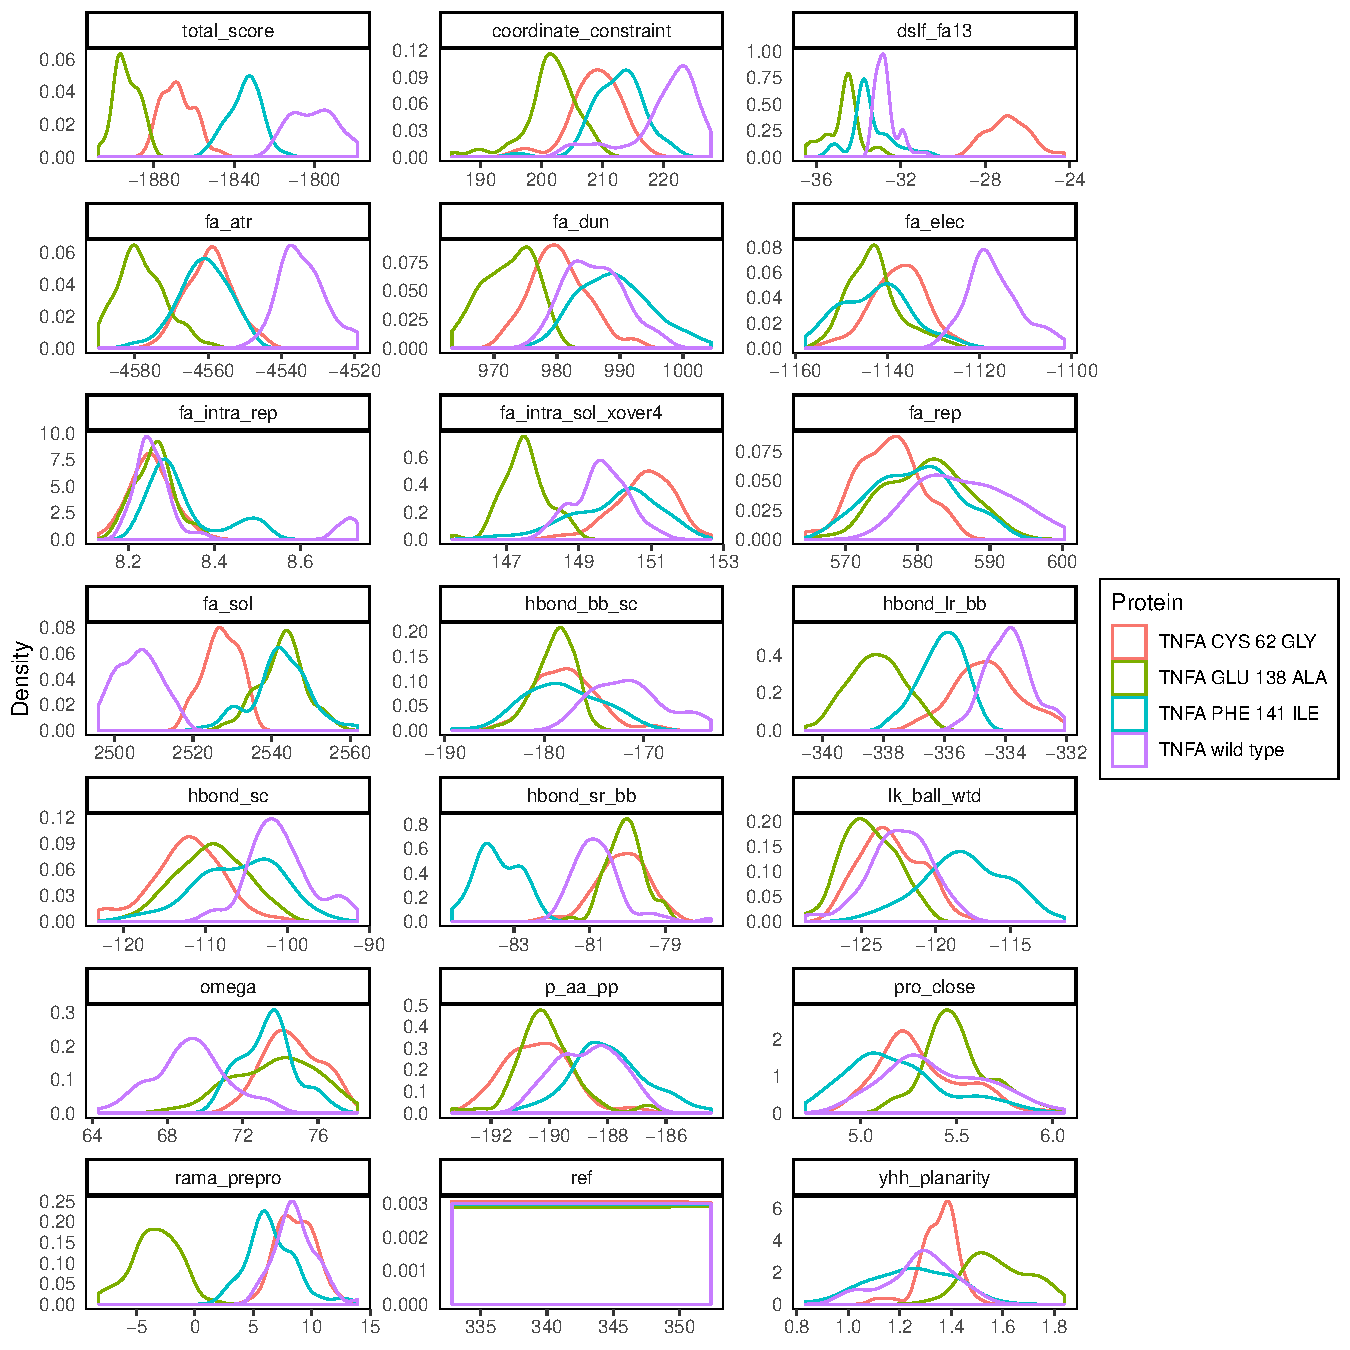
\includegraphics[width=\linewidth]{Rosetta_Backrub_Relax_Density_Plots/relax_Alpha_plot.pdf}
		\caption[TNFRSF1A homotrimer with TNF$\alpha$ homotrimer relax density plots]{Density of different scoring metrics from the models produced with relax of the wild type and all mutants that interacted with TNF$\alpha$. Most of the total scores, fa\_atr values and fa\_elec values of the mutated model are lower than the wild type that is bound to TNF$\alpha$ and the fa\_sol values are higher of the wild type than the mutants. TNFA CYS 62 GLY has more higher values at the dslf\_fa13 (disulfide geometry potential) than all other mutations. (Plots of backrub TNF$\alpha$ scores are in the supplementary.)(To zoom in on the details within the figure it is recommend to look at the PDF version.)}
		\label{fig:relax_TNFA_scores}
	\end{figure}

	\newpage
		
	\begin{figure}[!ht]
		\centering
		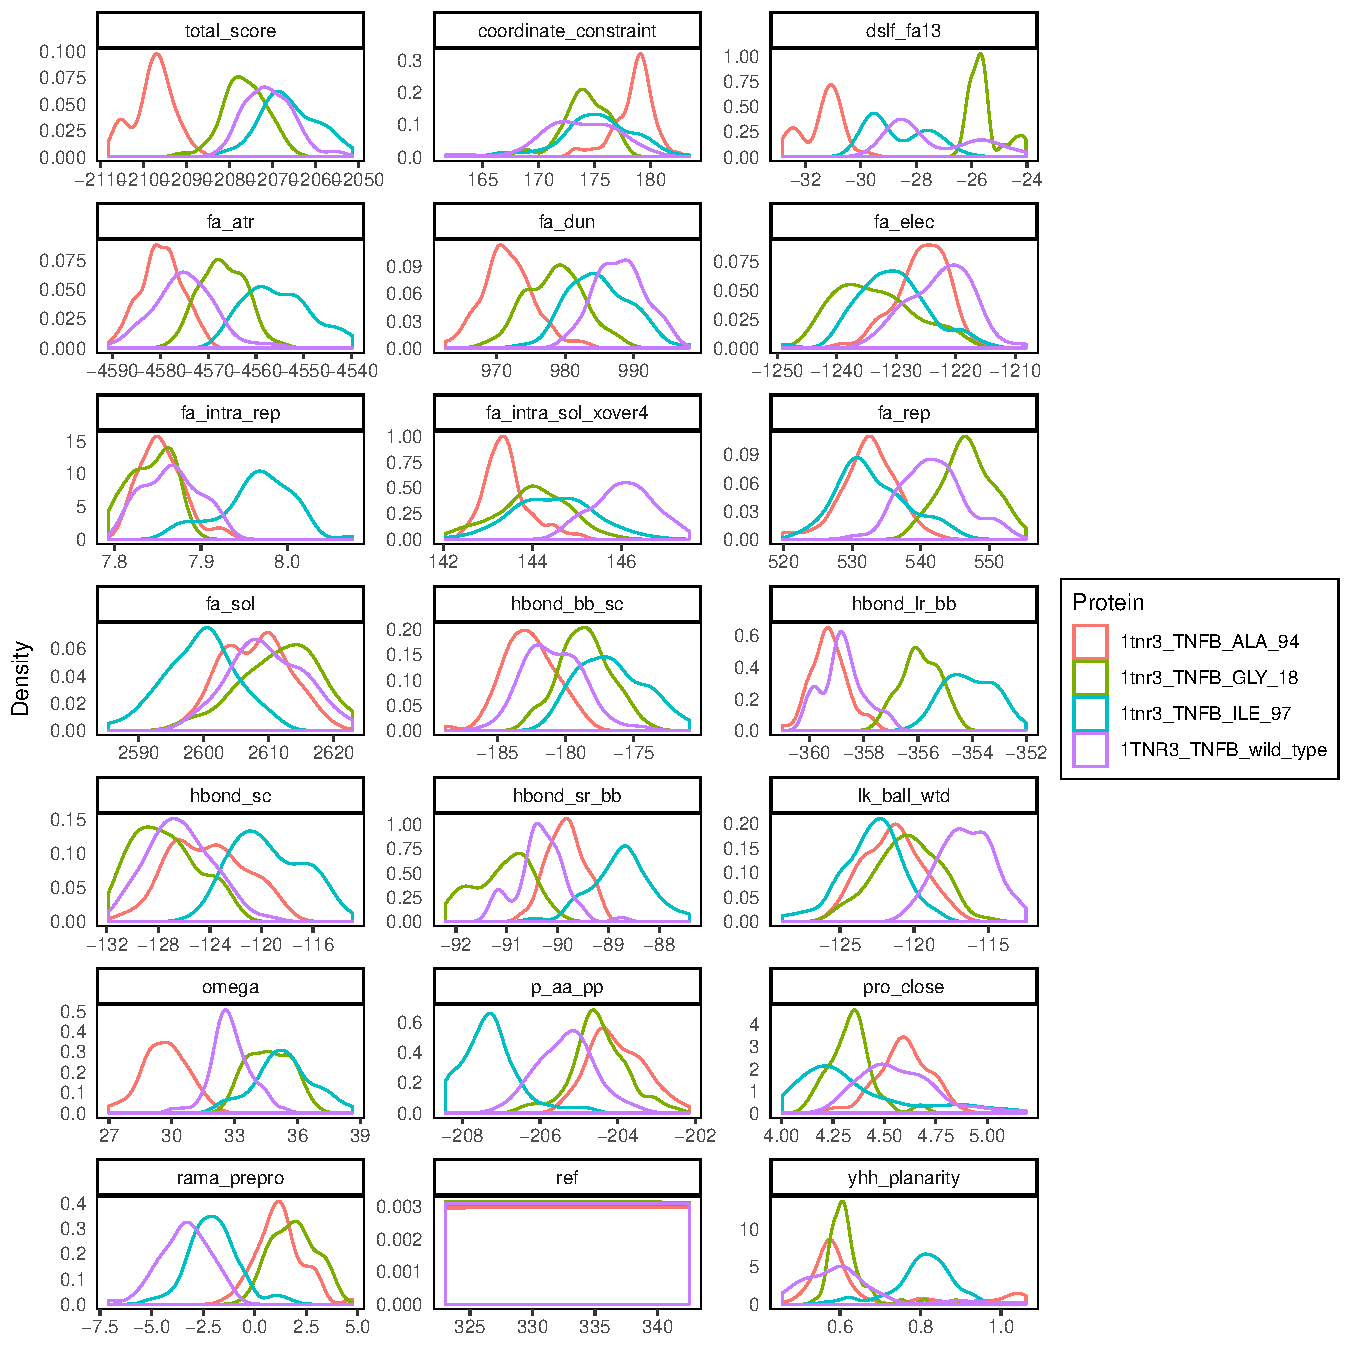
\includegraphics[width=\linewidth]{Rosetta_Backrub_Relax_Density_Plots/relax_Beta_plot.pdf}
		\caption[TNFRSF1A homotrimer with TNF$\beta$ homotrimer relax density plots]{Density distributions of the scores generated by relax for the wild type and mutations of TNFRSF1A that interact with TNF$\beta$. The total score values of TNFB GLU 138 ALA are lower than all other models and dslf\_fa13 (disulfide geometry potential) values are higher at TNFB CYS 62 GLY than the other models. fa\_intra\_rep (Lennard-Jones repulsive between atoms in the same residue) is higher within the models of PHE 141 ILE and hbond\_lr\_bb (Backbone-backbone hbonds distant in primary sequence) is higher at CYS 62 GLY and PHE 141 ILE.
		(Plots of backrub TNF$\beta$ scores are in the supplementary.)(To zoom in on the details within the figure it is recommend to look at the PDF version.)}
		\label{fig:relax_TNFB_scores}
	\end{figure}

	\newpage
	
	In the attempt to make mutated structures behave more natural two tools from the Rosetta software suite (Section \ref{subsec:MM_Rosetta}) had been used to minimize energies within protein structures. With the Backrub application (Section \ref{subsubsec:MM_Backrub}) 1000 altered backbone models have been produced each with 10000 Monte Carlo moves (Sections \ref{section:Chap_Monte_Carlo}). For each model that Backrub generated a set of scores were assigned to the properties, which together formed a collective score that described energy and bond occurrence in nature (Section \ref{subsec:MM_Rosetta}). Models of the wildtypes and mutants with the lowest collective score ,the best score, were chosen to undergo further side chain optimization within the Relax (Section \ref{subsubsec:MM_Relax}). 64 different relaxed models were produced and with various scores related to the properties of which the one with lowest total score would be chosen to visualize. 
	
	\begin{figure}[!ht]
		\centering
		\begin{subfigure}{0.49\textwidth}
			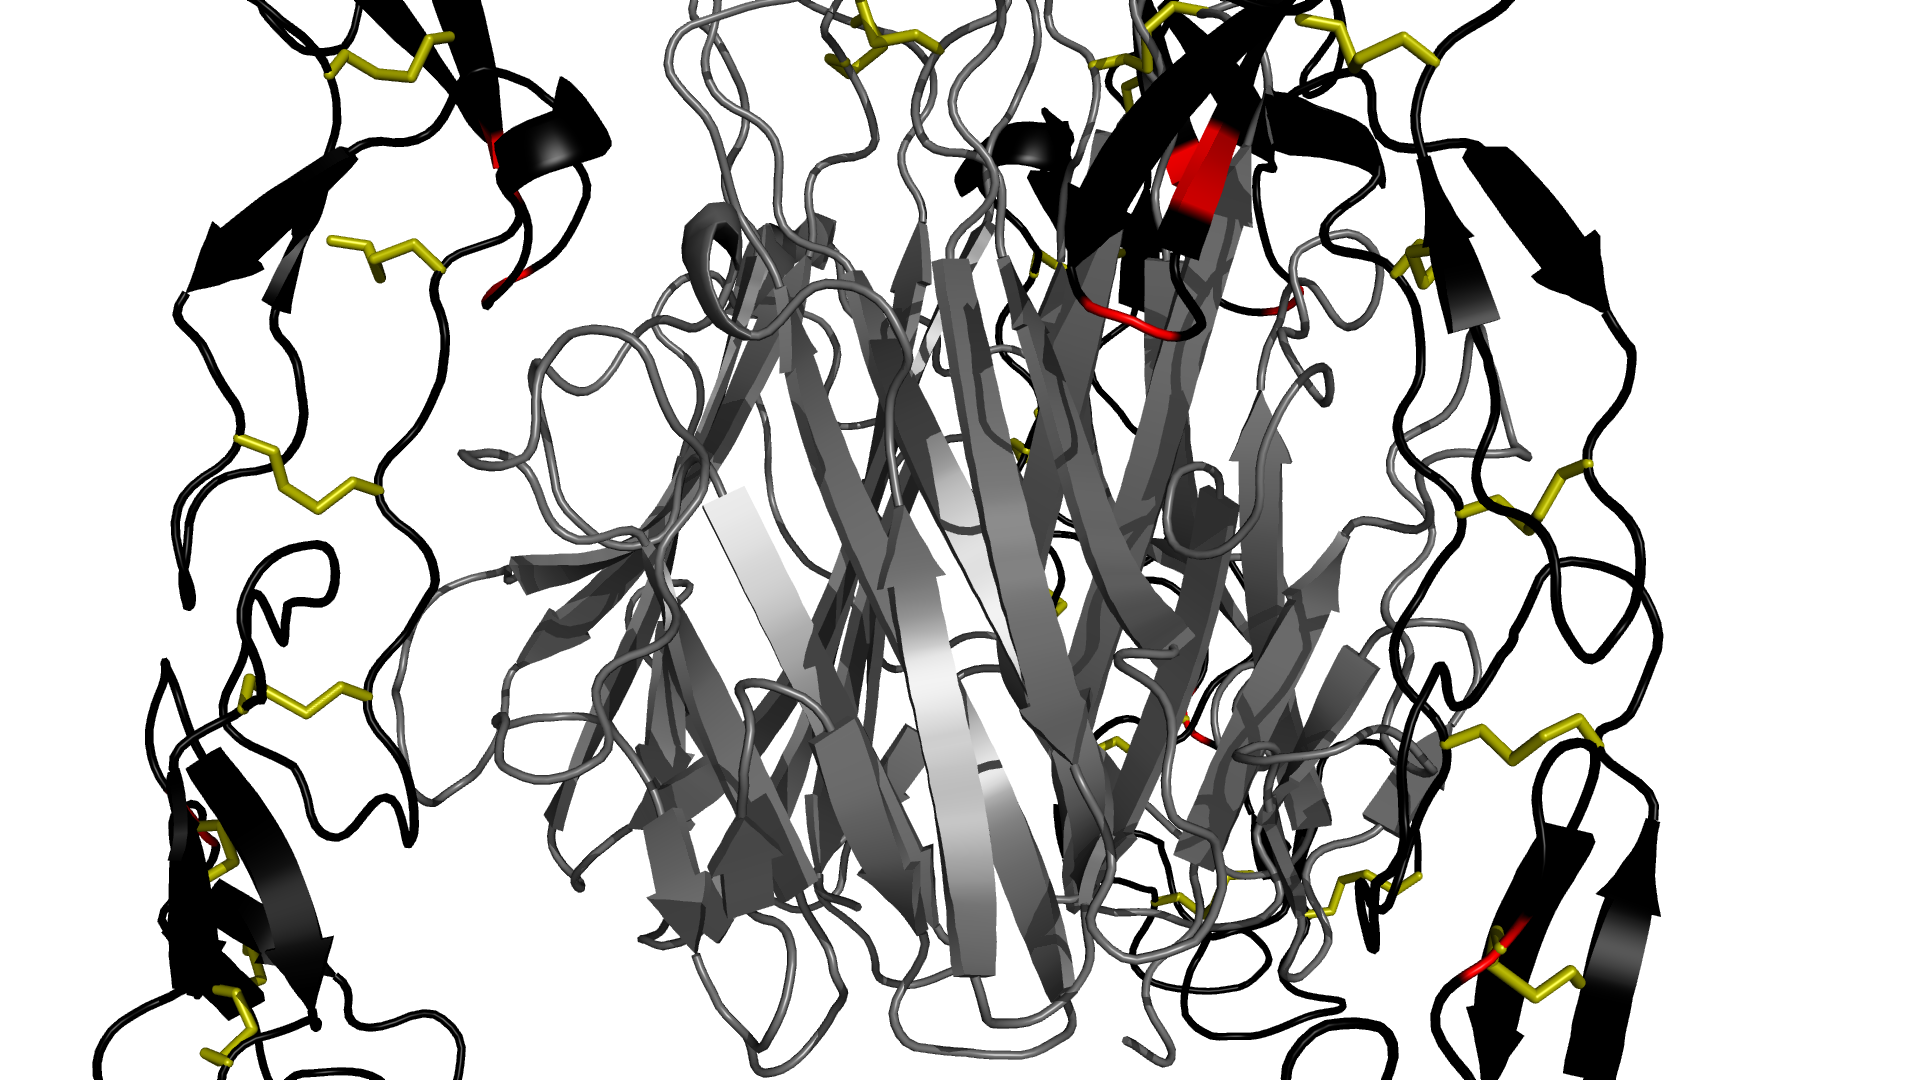
\includegraphics[width=\textwidth]{Relax_Pymol_Images/TNFA_wild.png}
			\caption{TNFRSF1A wild type with TNF$\alpha$}
			\label{fig:RES_TNFA_wild}
		\end{subfigure}
		\begin{subfigure}{0.49\textwidth}
			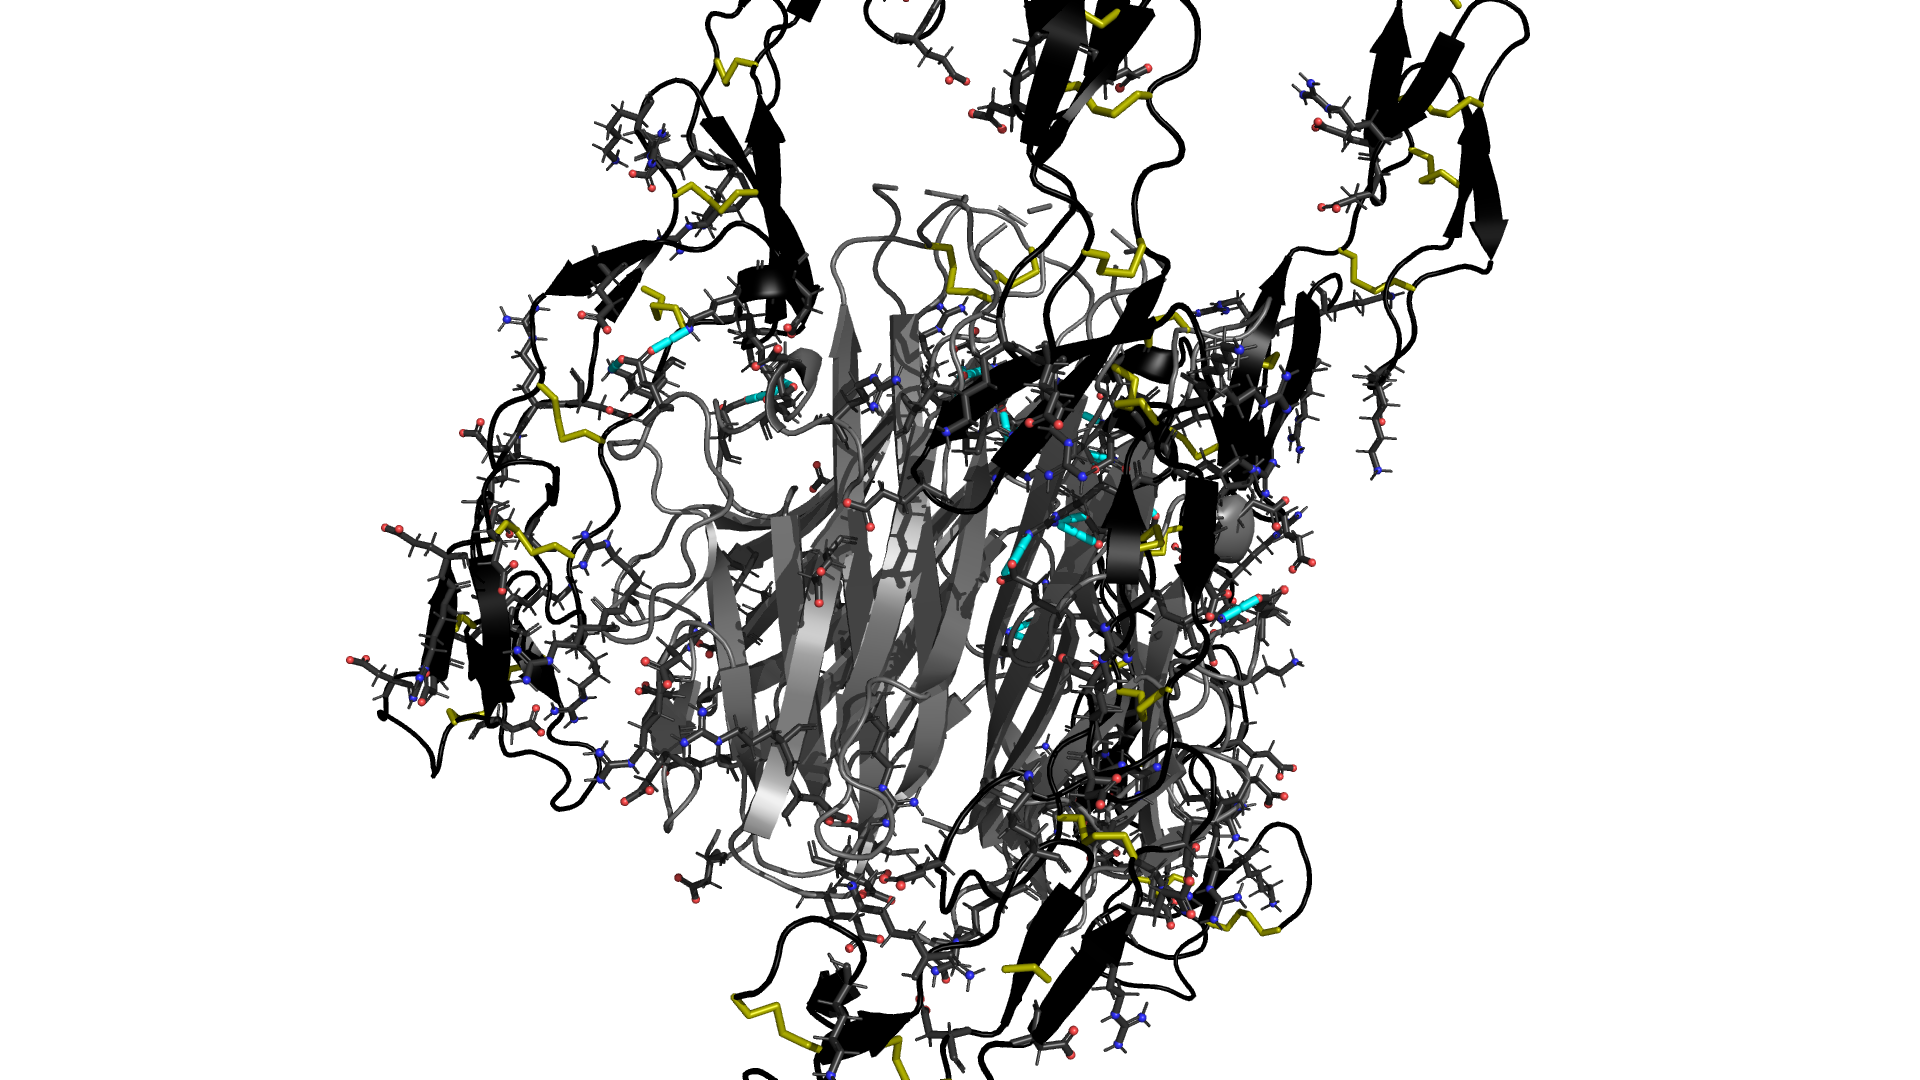
\includegraphics[width=\textwidth]{Relax_Pymol_Images/TNFA_18.png}
			\caption{TNFRSF1A CYS 62 GLY with TNF$\alpha$}
			\label{fig:RES_TNFA_18}
		\end{subfigure}
		\par\bigskip
		\begin{subfigure}{0.49\textwidth}
			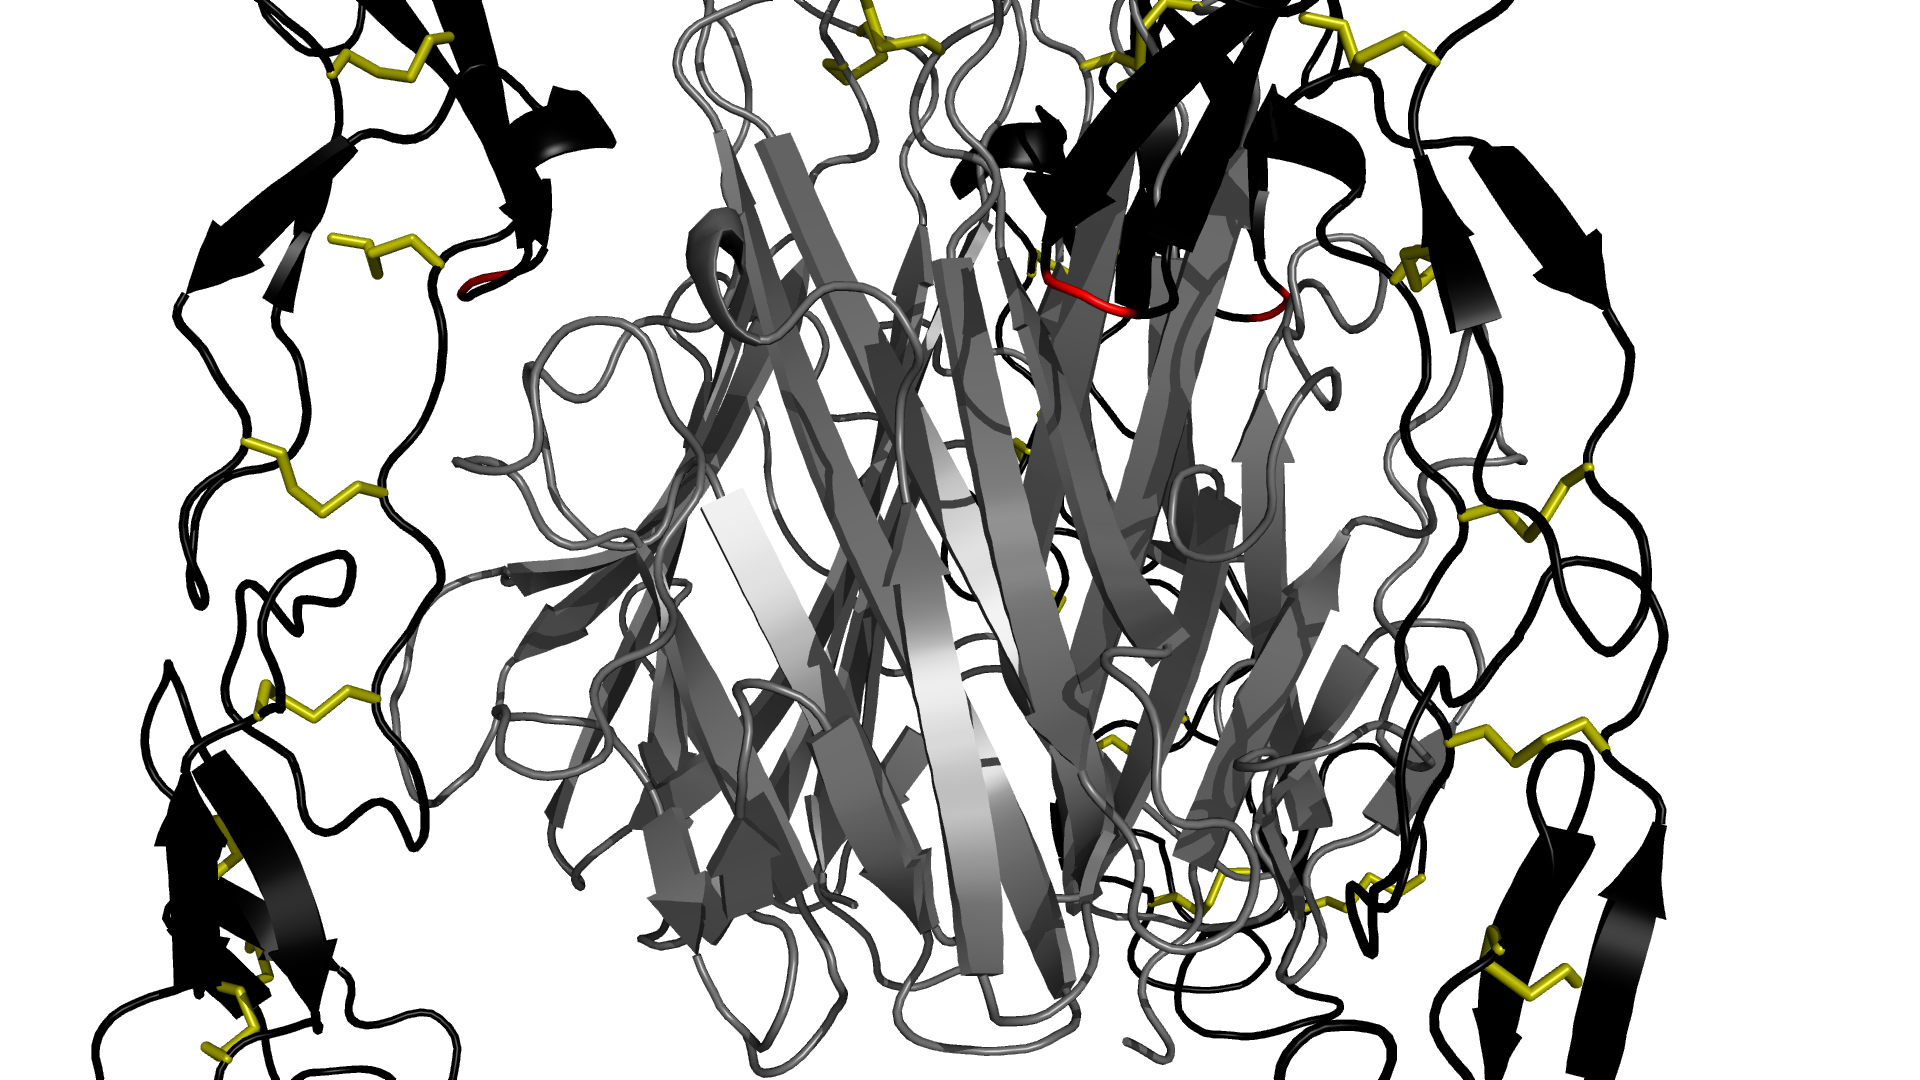
\includegraphics[width=\textwidth]{Relax_Pymol_Images/TNFA_94.png}
			\caption{TNFRSF1A GLU 138 ALA with TNF$\alpha$}
			\label{fig:RES_TNFA_94}
		\end{subfigure}
		\begin{subfigure}{0.49\textwidth}
			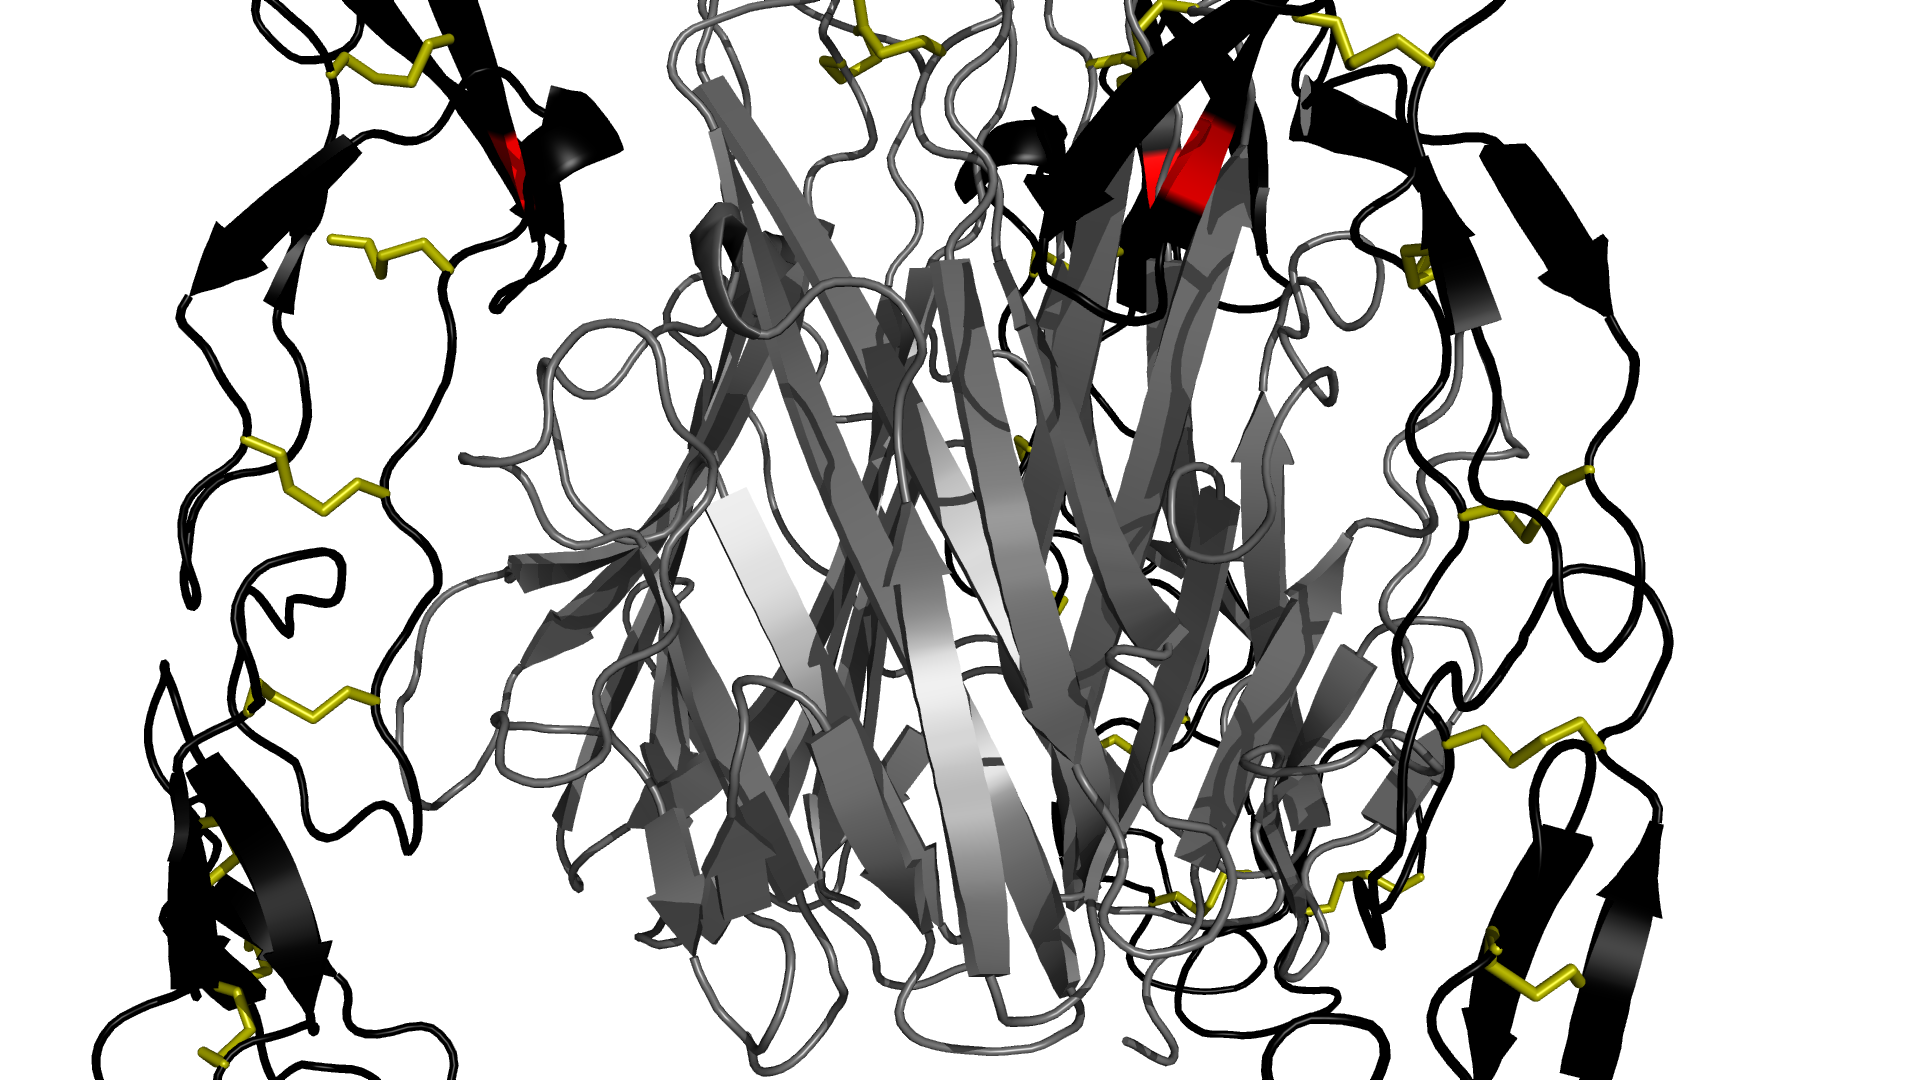
\includegraphics[width=\textwidth]{Relax_Pymol_Images/TNFA_97.png}
			\caption{TNFRSF1A PHE 141 ILE with TNF$\alpha$}
			\label{fig:RES_TNFA_97}
			\end{subfigure}
		\caption[TNFRSF1A homotrimer with TNF$\alpha$ homo trimers wild type and mutated relaxed models]{3D structures of a homotrimer TNFRSF1As (black) with a homotimer TNF$\alpha$s (gray) and disulfide bridges (dark yellow). The wild type (\ref{fig:RES_TNFA_wild}) has three red colored areas which are the original residues of the protein before any form of mutation. Within CYS 62 GLY (\ref{fig:RES_TNFA_18}) it is visible that at the position where a mutation is introduced (red) a disulfide bridge is missing. The mutations of GLU 138 ALA (\ref{fig:RES_TNFA_94}) and PHE 141 ILE (\ref{fig:RES_TNFA_97}) show no large differences at the mutated spots (red).(To zoom in on the details within the figure it is recommend to look at the PDF version.)}
		\end{figure}
		\newpage
		
		\begin{figure}[!ht]
		\centering
		\begin{subfigure}{0.49\textwidth}
			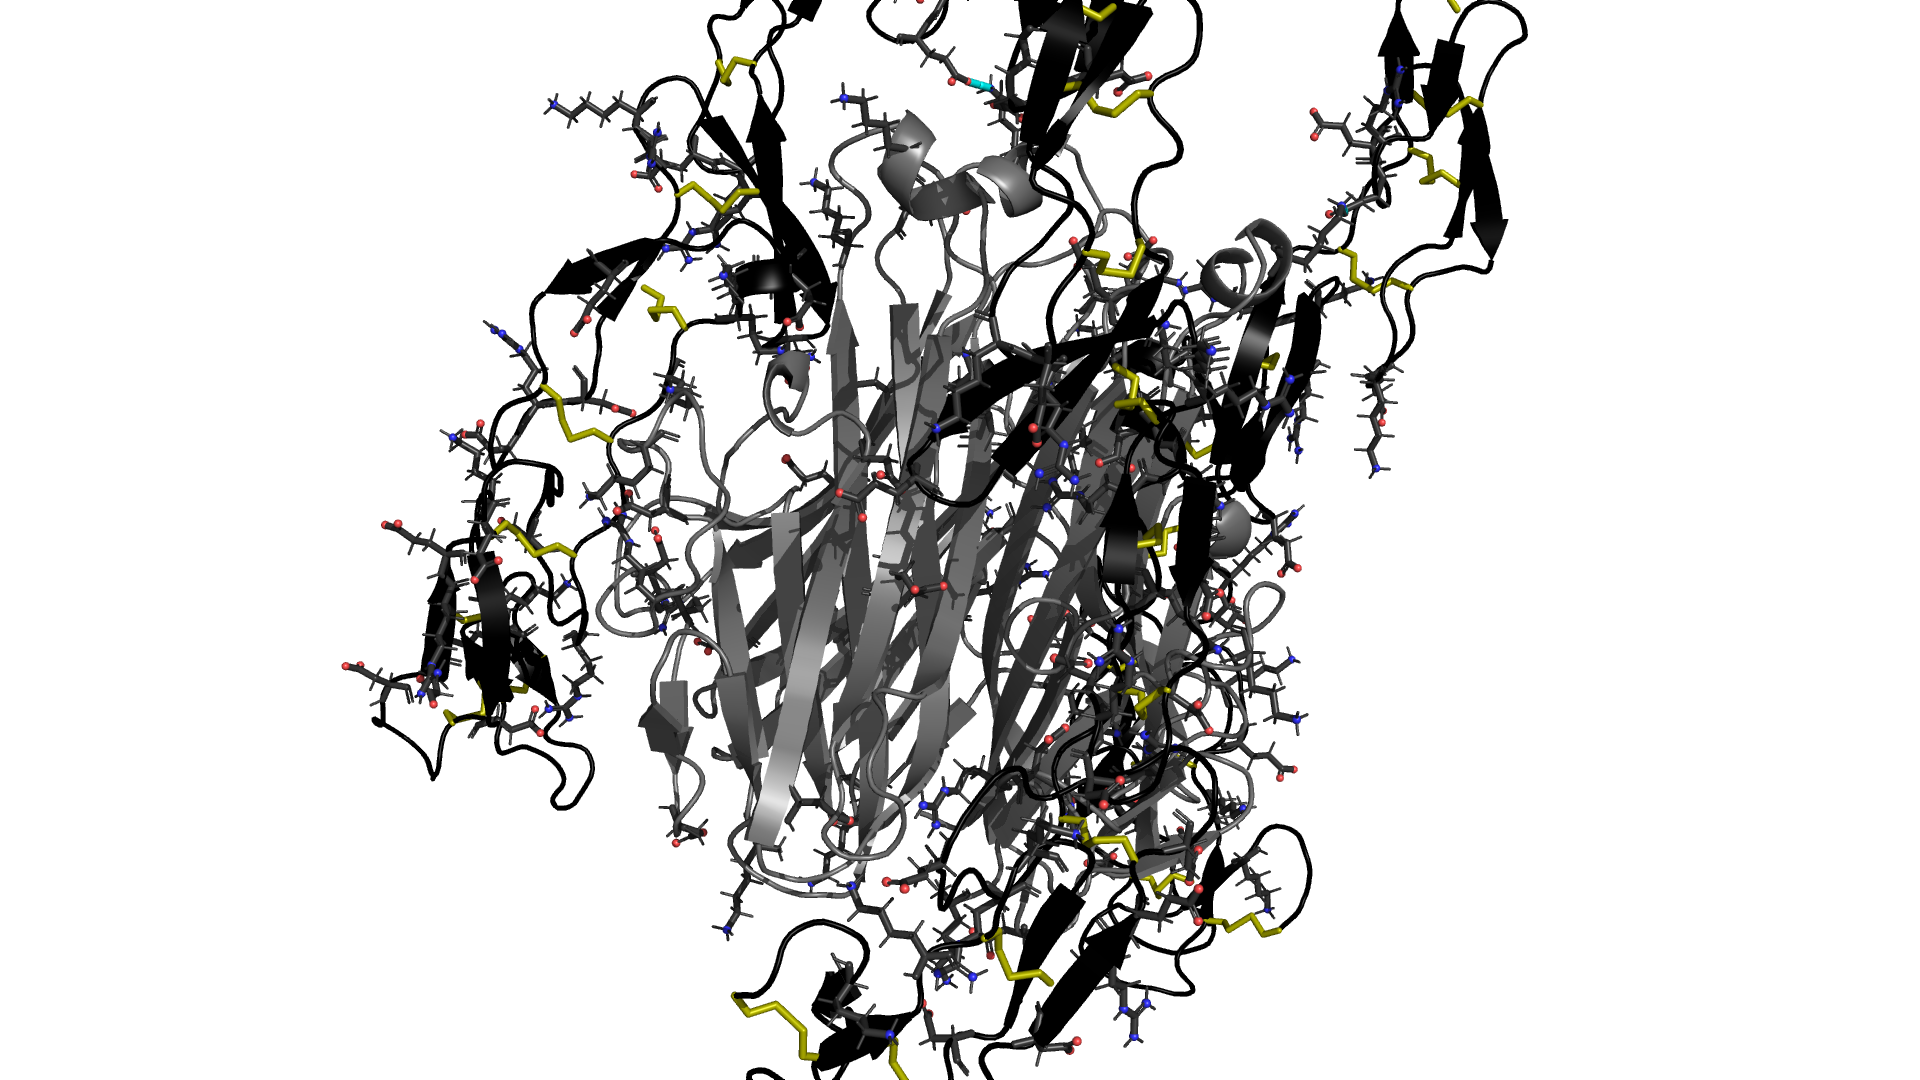
\includegraphics[width=\textwidth]{Relax_Pymol_Images/TNFB_wild.png}
			\caption{TNFRSF1A wild type with TNF$\beta$}
			\label{fig:RES_TNFB_wild}
		\end{subfigure}
		\begin{subfigure}{0.49\textwidth}
			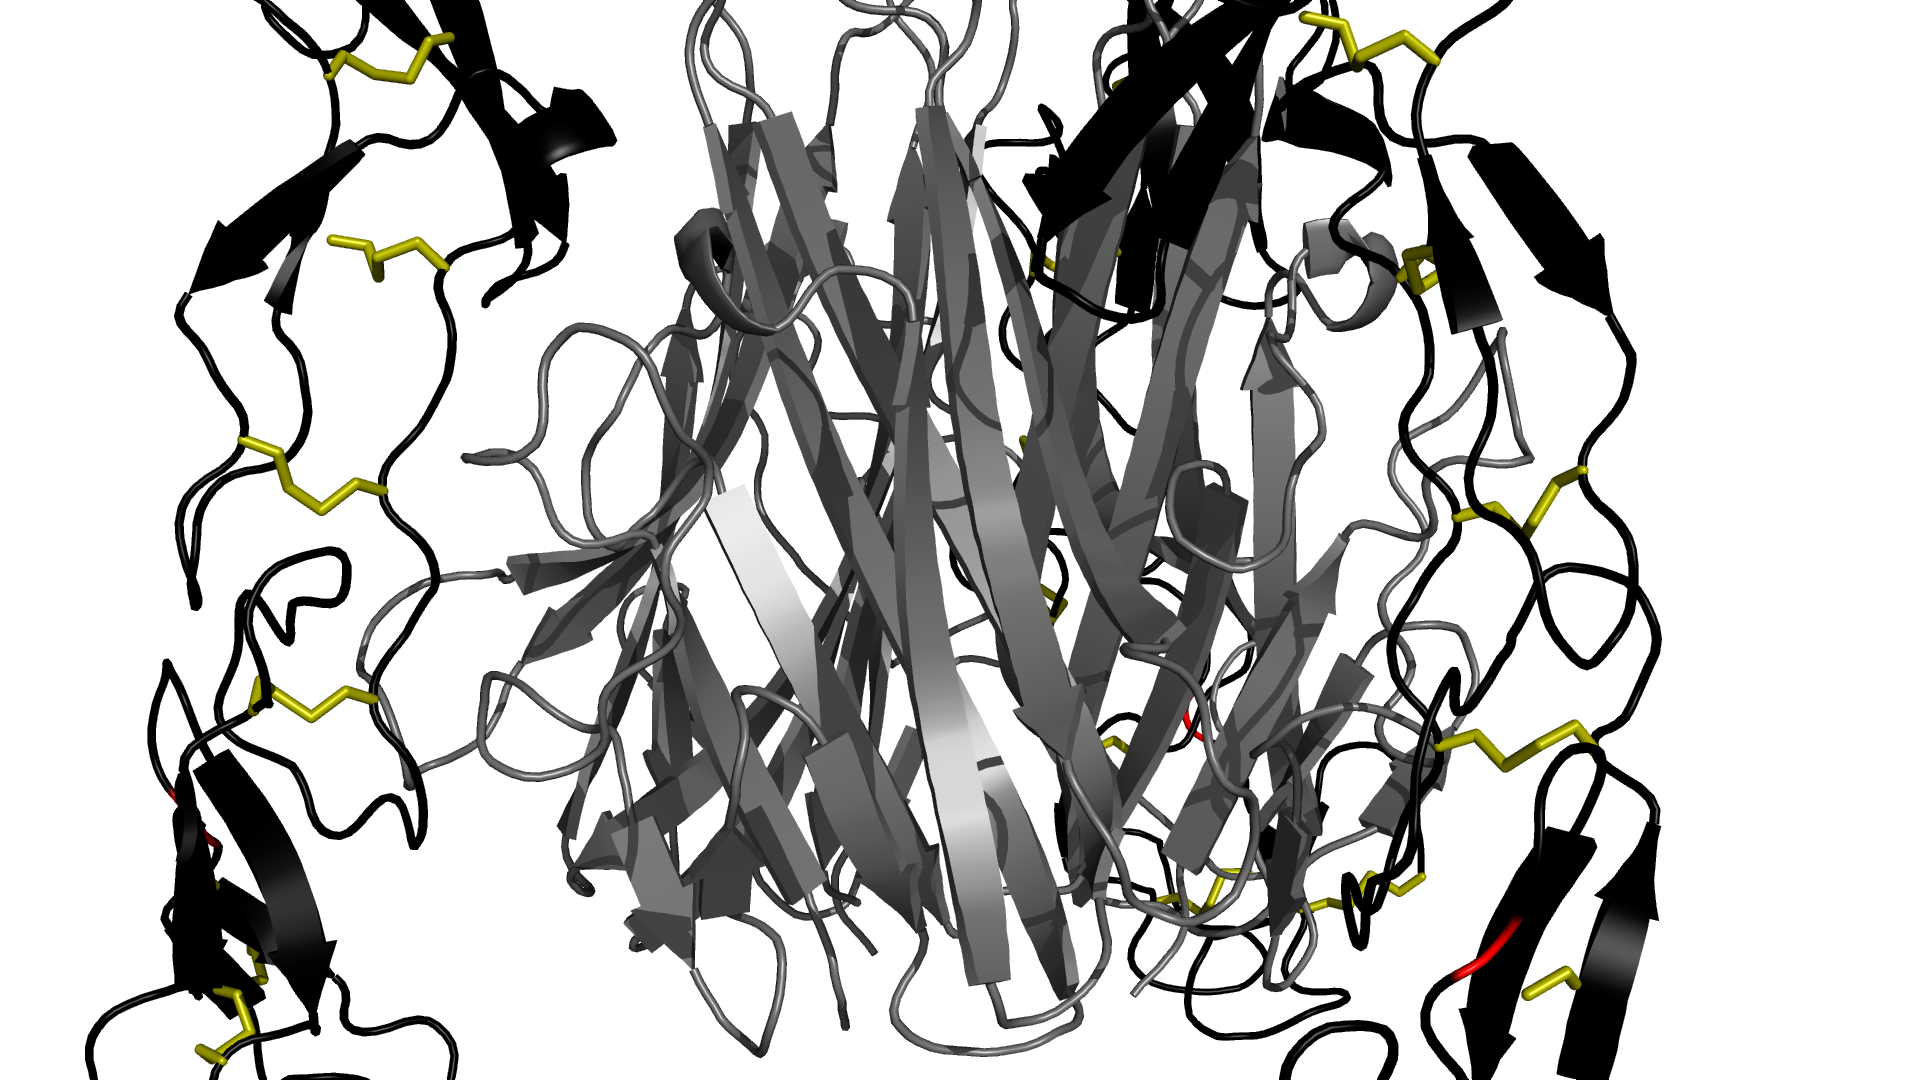
\includegraphics[width=\textwidth]{Relax_Pymol_Images/TNFB_18.png}
			\caption{TNFRSF1A CYS 62 GLY with TNF$\beta$}
			\label{fig:RES_TNFB_18}
		\end{subfigure}
		\par\bigskip
		\begin{subfigure}{0.49\textwidth}
			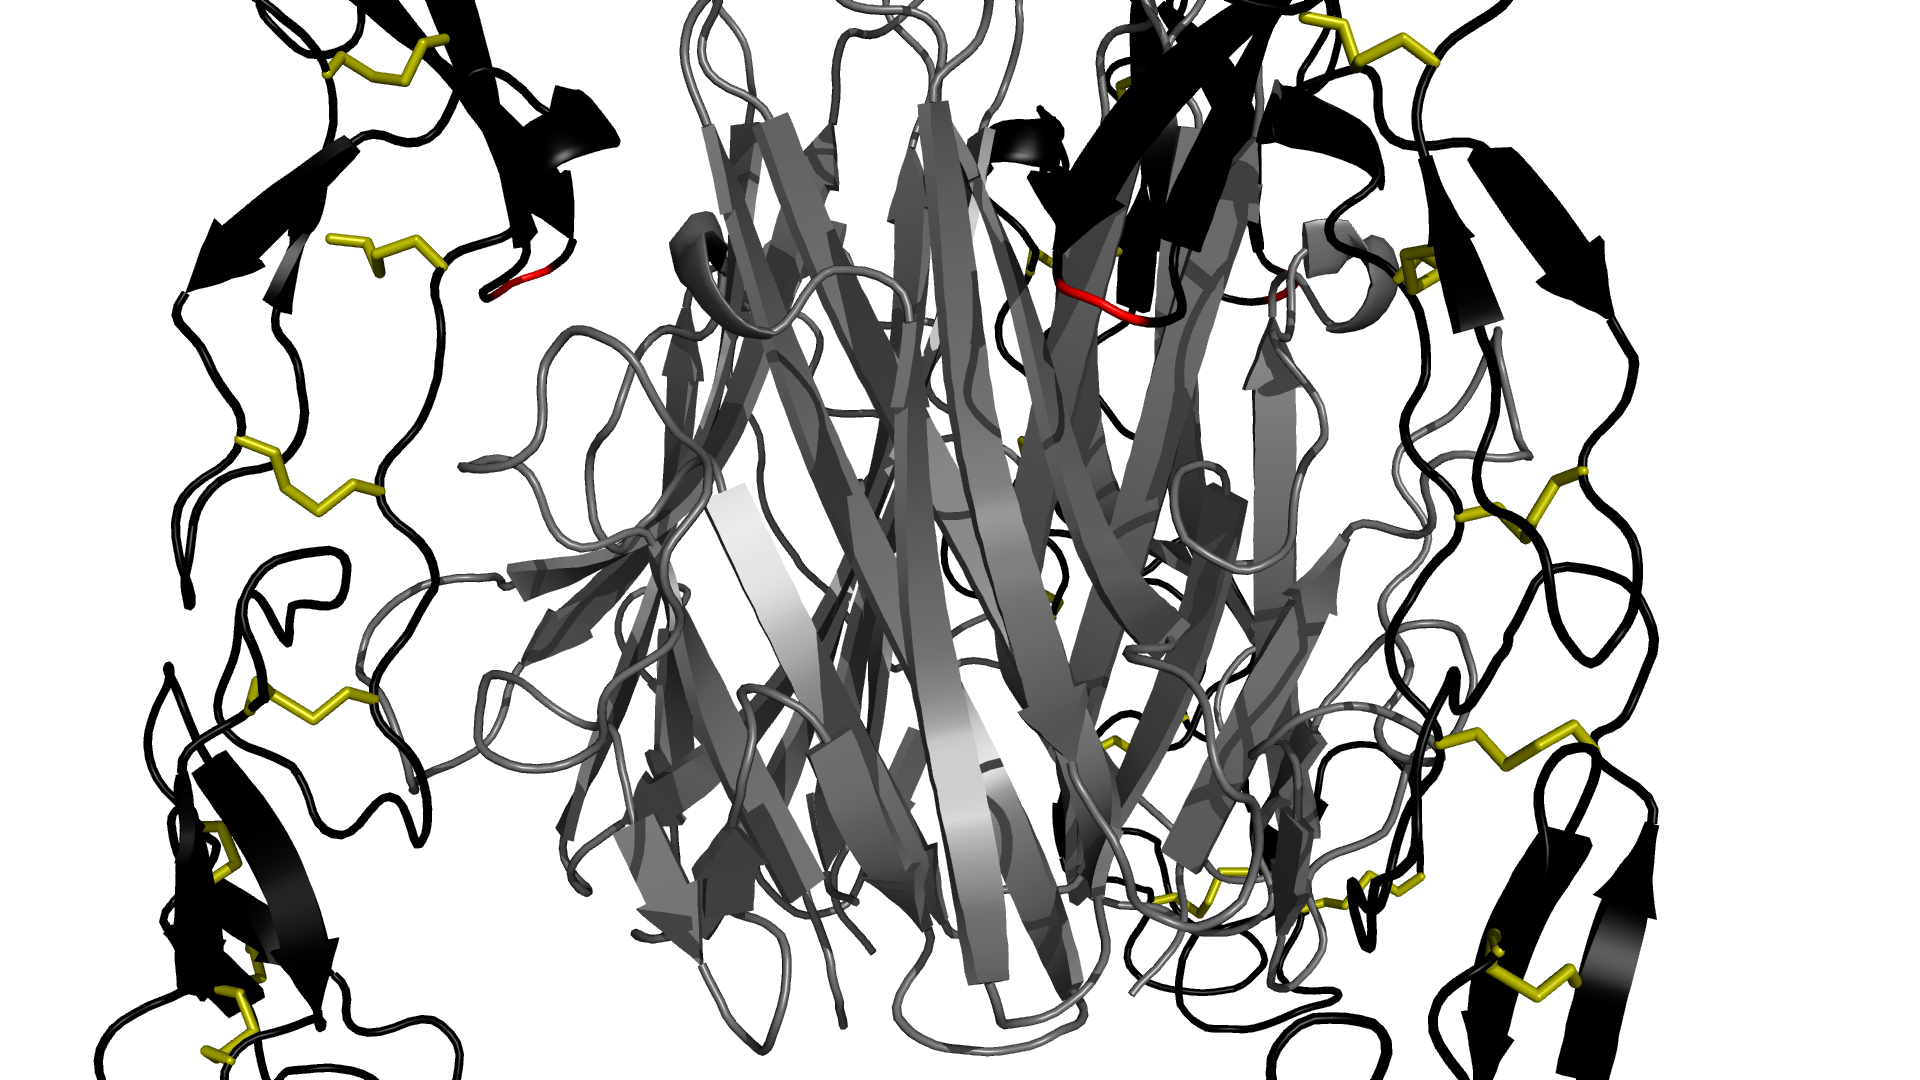
\includegraphics[width=\textwidth]{Relax_Pymol_Images/TNFB_94.png}
			\caption{TNFRSF1A GLU 138 ALA with TNF$\beta$}
			\label{fig:RES_TNFB_94}
		\end{subfigure}
		\begin{subfigure}{0.49\textwidth}
			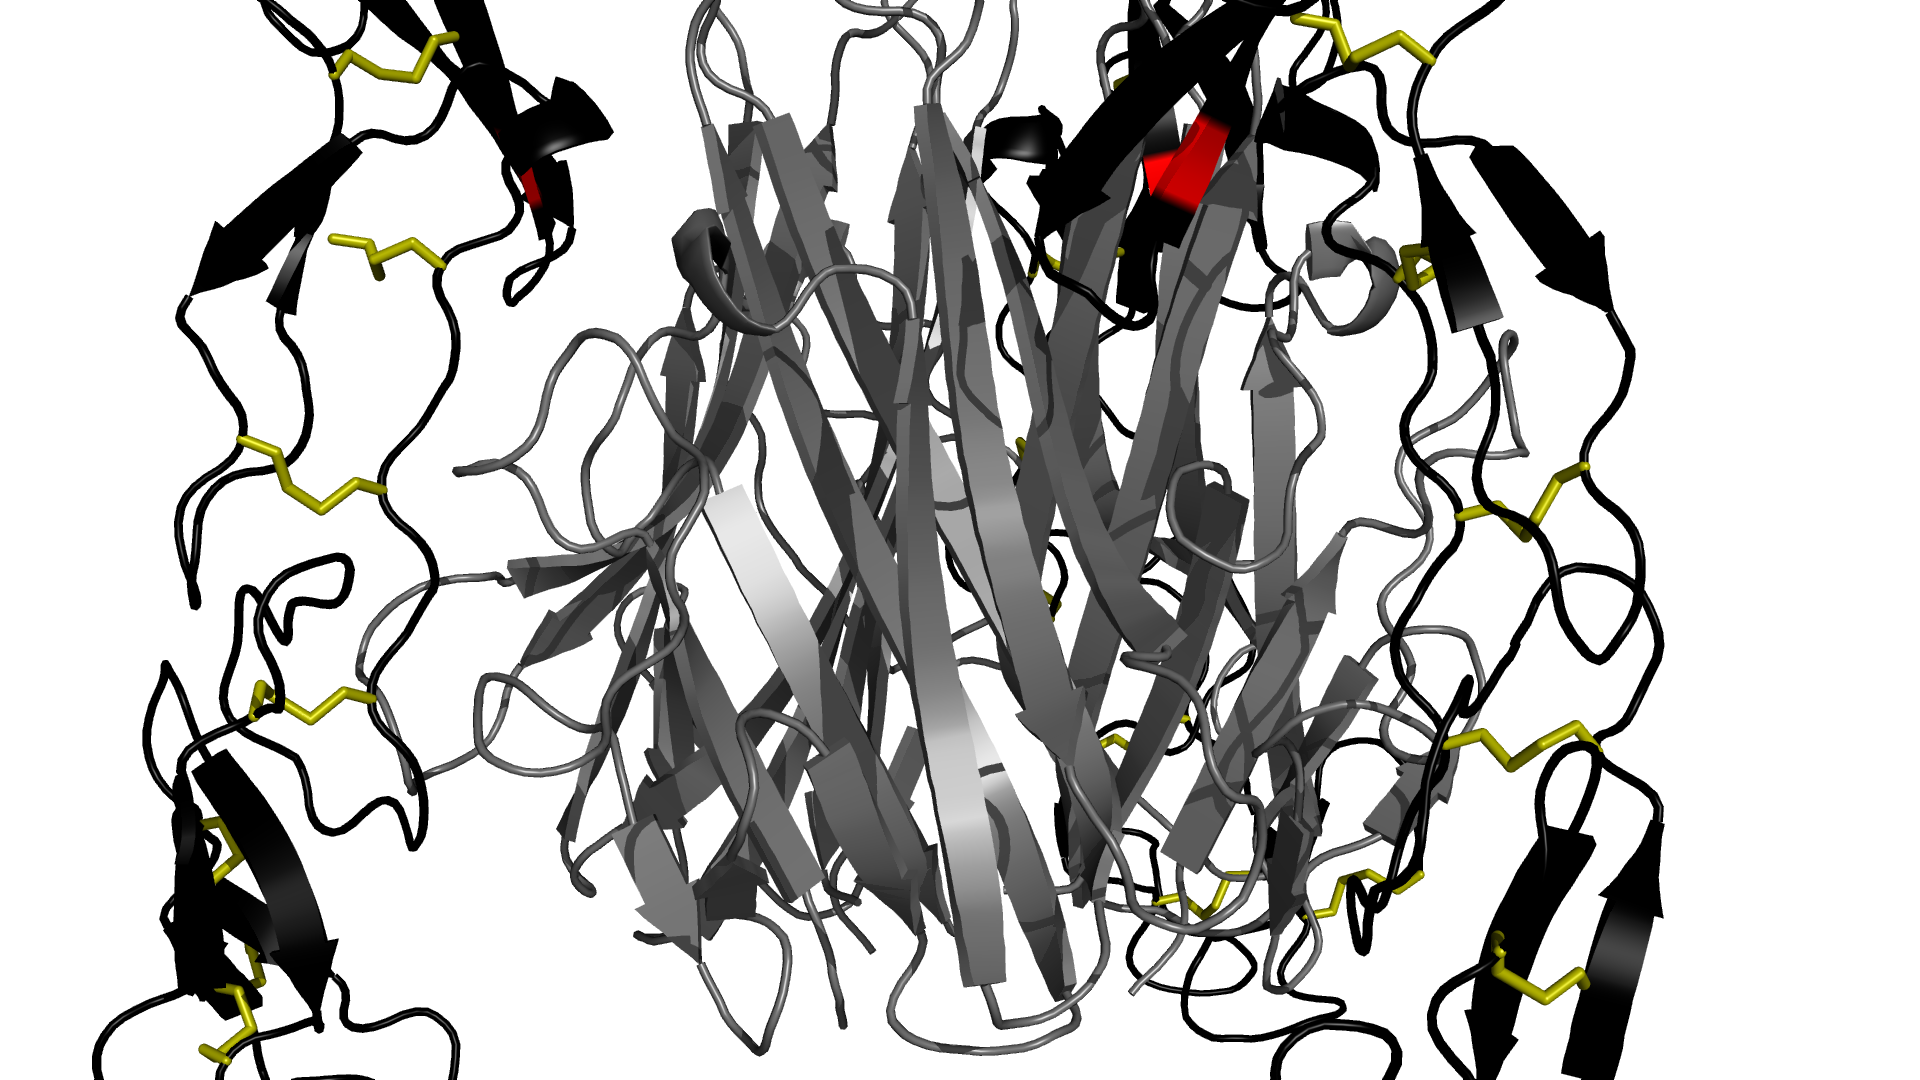
\includegraphics[width=\textwidth]{Relax_Pymol_Images/TNFB_97.png}
			\caption{TNFRSF1A PHE 141 ILE with TNF$\beta$}
			\label{fig:RES_TNFB_97}
		\end{subfigure}
	\caption[TNFRSF1A homotrimer with TNF$\beta$ homo trimers wild type and mutated relaxed models]{3D structures of a homotrimer TNFRSF1As (black) with a homotimer TNF$\beta$s (gray) and disulfide bridges (dark yellow). The wild type (\ref{fig:RES_TNFB_wild}) has three red colored areas which are the original residues of the protein before any form of mutation. Within CYS 62 GLY (\ref{fig:RES_TNFB_18}) it is visible that at the position where a mutation is introduced (red) a disulfide bridge is missing. The mutations of GLU 138 ALA (\ref{fig:RES_TNFB_94}) and PHE 141 ILE (\ref{fig:RES_TNFB_97}) show no large differences at the mutated spots (red).(To zoom in on the details within the figure it is recommend to look at the PDF version.)}
	\end{figure}
	
\newpage
	
\newpage	
\subsection{Finding mutation information with HOPE}
	With uncertainty in the numbers provided by SPVAA a more textual informative approach was used with the web service HOPE (Section \ref{subsec:MM_HOPE}). The mutations that were known from Infevers (Section \ref{subsec:MM_Infevers}) and were also used with SPVAA were tested by HOPE (CYS62GLY, GLU138ALA and PHE141IlE), all reports are visible within the supplementary.
	
	HOPEs first test was the mutation of Cysteine 62 to glycine, which is known within the Infevers table as pathogenic and was validated. It discovered that the residue was involved in a disulfide bridge and was 100\% conserved in related protein sequences, based on the observation that cysteine formed a disulfide bridge it expected that with te replacement of it glycine would make the whole structures less rigid. HOPE predicts that mutation is pathogenic because of the high conservation of the residue, which is further confirmed by its search results in which if found the original publication where the observation has been described and associated to TRAPS \cite{aksentijevich_tumor-necrosis-factor_2001}.
%	The tumor-necrosis-factor receptor-associated periodic syndrome: new mutations in TNFRSF1A, ancestral origins, genotype-phenotype studies, and evidence for further genetic heterogeneity of periodic fevers, Aksentijevich
	
	According to Infevers is the mutation of glutamic acid at position 138 mutated to alanine classified as likely benign and was not validated yet. HOPE discovered with a BLAST query that glutamic acid occurs often at position but other residues such as alanine have been observed at the position. Structurally glutamic acid forms salt bridges with proline  368 and leucine 390 and is found in a sequence of amino acids that is repeated through out TNFRSF1A. The amino acid lies within a domain where it interacts with other domains and is important for the proteins activity, with this mutation it might already perturb the binding capabilities according to HOPE.
	
	The last mutation that was tested with HOPE was phenylalanine 141 to Isoleucine and was according to Infevers pathogenic and has been validated. Phenylalanine has been conserved at this positions and few other residues have been seen at the position, it is member of the identical domain as glutamic acid 138 and HOPE predicts that it would not damage the protein based on this information. However within the structure it could inhibit interaction with other domains and protein activity.
	
	
%	
%	
%	 to arrange this information properly a Python script (Section \ref{subsec:MM_Python}) used the files and
%	
%	 and the exact position within the PDB file (1TNR) had to be added with a Python script (Section \ref{})
%	
%	 were introduced with a Python script (Section \ref{subsec:MM_Python}) wherein  and had to be introduced with  Introducing mutations in the trimeric mol
%	
%	Each of wherein mutated 
%	
%	
%	
%	three mutations in separate structures were introduced.
%	
%	The mutation tables first column is insufficient and requires additional information regarding TNFRSF1A chains to make mutations in TNFRSF1A, information regarding the chains 
%	
%	From the mutation table only information of the first column is used to make alterations in structural models, that part of the table will play a role in modifying protein structures with Modeller (Section \ref{subsec:MM_Modeller}). Because the model is homotrimeric it has multiple poly peptides chains that all need to be modified without modifying the ligand. 
%	
%		
%	
%	 But more information is required to make a new format, since TNFRSF1A is a homotimer a
%	the function of the mutated protein is within a pathway 
%	A broad perspective should be taken with a 
%	To determine the effects of mutated residue awithin a protein variant a b than structural information should
%	Up until VIPUR and the development of similar approaches that benefit from structural information

%
%
%
%Something about that we tried to use the VTS and add our protein for information.



